\documentclass[11pt]{article}
\usepackage[utf8]{inputenc}
\usepackage[spanish]{babel}
\decimalpoint
\usepackage{amsmath}
\usepackage{amsthm}
\usepackage{amssymb}
\usepackage{graphicx}
\usepackage[margin=0.8in]{geometry}
\usepackage{fancyhdr}
\usepackage[inline]{enumitem}
\usepackage{float}
\usepackage{cancel}
\usepackage{bigints}
\usepackage{listings}
\usepackage{xcolor}
\usepackage{listingsutf8}
\usepackage{algpseudocode}
\usepackage{algorithm}
\usepackage{apacite}
\usepackage{tcolorbox}
\usepackage{multicol}
\usepackage{tipa}
\usepackage{caption} 
\pagestyle{fancy}
\usepackage{hyperref}
\usepackage{mathtools}% http://ctan.org/pkg/mathtools

\hypersetup{
    colorlinks,
    citecolor=black,
    filecolor=black,
    linkcolor=black,
    urlcolor=black
}
\newcommand{\xvdash}[1]{%
	\vdash^{\mkern-10mu\scriptscriptstyle\rule[-.9ex]{0pt}{0pt}#1}%
}
\setlength{\headheight}{15pt} 
\lhead{Tarea 7. Desarrollo de un cliente para un servicio web estilo REST}
\rhead{\thepage}
\lfoot{ESCOM-IPN}
\renewcommand{\footrulewidth}{0.5pt}
\setlength{\parskip}{0.5em}
\newcommand{\ve}[1]{\overrightarrow{#1}}
\newcommand{\abs}[1]{\left\lvert #1 \right\lvert}
\newcommand{\blank}{\text{\textcrb}}
\date{\today}
\title{Tarea 7. Desarrollo de un cliente para un servicio web estilo REST}
\author{Sanchez Mendez Edmundo Josue}

\lstset{
tabsize = 4, %% set tab space width
showstringspaces = false, %% prevent space marking in strings, string is defined as the text that is generally printed directly to the console
numbers = left, %% display line numbers on the left
commentstyle = \color{green}, %% set comment color
keywordstyle = \color{blue}, %% set keyword color
stringstyle = \color{red}, %% set string color
rulecolor = \color{black}, %% set frame color to avoid being affected by text color
basicstyle = \small \ttfamily , %% set listing font and size
breaklines = true, %% enable line breaking
numberstyle = \tiny,
}

\bibliographystyle{apacite}
\begin{document}
		\begin{titlepage}
			\begin{center}
				
				% Upper part of the page. The '~' is needed because \\
				% only works if a paragraph has started.
				
				\noindent
				\begin{minipage}{0.5\textwidth}
					\begin{flushleft} \large
						
\includegraphics[width=0.5\textwidth]{resources/ipn.png}
					\end{flushleft}
				\end{minipage}%
				\begin{minipage}{0.55\textwidth}
					\begin{flushright} \large
						
\includegraphics[width=0.5\textwidth]{resources/escom.png}
					\end{flushright}
				\end{minipage}
				
				\textsc{\LARGE Instituto Politécnico Nacional}\\[0.5cm]
				
				\textsc{\Large Escuela Superior de Cómputo}\\[1cm]
				
				% Title
				
				{ \huge Tarea 7. Desarrollo de un cliente para un servicio web estilo REST \\[1cm] }
				
				{ \Large Unidad de aprendizaje: Desarrollo de Sistemas Distribuidos} \\[1cm]
				
				{ \Large Grupo: 4CV11 } \\[1cm]
				
				\noindent
				\begin{minipage}{0.5\textwidth}
					\begin{flushleft} \large
						\emph{Alumno:} \\
						Sanchez Mendez Edmundo Josue
					\end{flushleft}
				\end{minipage}%
				\begin{minipage}{0.5\textwidth}
					\begin{flushright} \large
						\emph{Profesor:} \\
						Pineda Guerrero Carlos 
					\end{flushright}
				\end{minipage}
				
				\vfill
				% Bottom of the page
				{\large {\today}}
			\end{center}
		\end{titlepage}
	
	\titlepage
	\tableofcontents
	\newpage
	
	\section{Introducción}
		Desarrollar un programa Java consola (modo carácter) cliente del servicio web REST que se implemento en la tarea anterior. Se deberá realizar las siguientes modificaciones al servicio web:
		\begin{itemize}
			\item Agregar el campo id\_usuario a la clase Usuario (Usuario.java).
			\item Modificar el método web ``alta\_usuario`` (Servicio.java), de manera que al dar de alta un usuario el método web deberá regresar al cliente el id del usuario agregado. Se deberá desplegar el id del usuario dado de alta. El campo id\_usuario es auto\_increment en la base de datos, por tanto se deberá recuperar el ID inmediatamente después de ejecutar la instrucción INSERT.
			\item Modificar el método web ``consulta\_usuario`` (Servicio.java), ahora la consulta se deberá realizar mediante el id del usuario no el email.
			\item Modificar el método web ``modifica\_usuario`` (Servicio.java), utilizar el id del usuario en el WHERE de las instrucciones SQL en lugar del email. No deberá modificar el id de un usuario ya que se trata de la llave primaria.
			\item Modificar el método web ``borra\_usuario`` (Servicio.java), utilizando como clave el id del usuario no el email.
		\end{itemize}
		El programa cliente deberá desplegar el siguiente menú:\par
		MENU\par
a. Alta usuario\par
b. Consulta usuario\par
c. Borra usuario\par
d. Salir\par
\par
Opción: \_\par

Las opciones deberán implementar la siguiente funcionalidad:
\begin{itemize}
			\item La opción ``Alta usuario`` leerá del teclado el email, el nombre del usuario, el apellido paterno, el apellido materno, la fecha de nacimiento, el teléfono y el género (``M`` o ``F``). Entonces se invocará el método web ``alta\_usuario``. Se deberá desplegar el id del usuario dado de alta, o bien, el mensaje de error que regresa el servicio web. Notar que el método web ``alta\_usuario`` recibe como parámetro una instancia de la clase Usuario, recordemos que esta clase se deberá definir de la siguiente manera:
			\begin{verbatim}
			class Usuario
    {
      int id_usuario;
      String email;
      String nombre;
      String apellido_paterno;
      String apellido_materno;
      String fecha_nacimiento;
      String telefono;
      String genero;
      byte[] foto;
    }
		\end{verbatim}
		\end{itemize}
Para invocar el método web ``alta\_usuario`` desde el cliente Java es necesario crear una instancia de la clase Usuario y asignar los valores a los campos (en este caso el campo ``foto`` será null). Una vez que se tenga el objeto de tipo Usuario se deberá utilizar GSON para convertir el objeto a una string JSON, entonces se deberá codificar como URL y el resultado se utilizará como valor del parámetro.
\begin{itemize}
			\item La opción ``Consulta usuario`` leerá del teclado el id de un usuario previamente dado de alta. Entonces se invocará el método web ``consulta\_usuario``. Si el usuario existe, se desplegará en pantalla el nombre del usuario, el apellido paterno, el apellido materno, la fecha de nacimiento, el teléfono y el género. Debido a que el programa no es gráfico, la foto del usuario se ignorará. Notar que el método web ``consulta\_usuario`` regresa una string JSON la cual representa un objeto de tipo Usuario, por tanto será necesario utilizar GSON para convertir la string JSON a un objeto Java de tipo Usuario y posteriormente desplegar los campos del objeto (excepto el campo ``foto``). Si hubo error, se desplegará el mensaje que regresa el servicio web. Una vez desplegados los datos del usuario se preguntará ``¿Desea modificar los datos del usuario (s/n)?``, si se responde con un caracter ``s`` entonces se leerá del teclado el email, el nombre del usuario, el apellido paterno, el apellido materno, la fecha de nacimiento, el teléfono y el género (``M`` o ``F``), si un campo se presiona solo Enter, entonces el campo queda sin modificar.  Entonces se invocará el método web ``modifica\_usuario``. Este método recibe como parámetro un objeto de tipo Usuario, por tanto se deberá utilizar GSON para convertir el objeto a una string JSON, entonces se deberá codificar como URL y el resultado se utilizará como valor del parámetro. Se deberá desplegar ``El usuario ha sido modificado`` si se pudo modificar el usuario, o bien, el mensaje de error que regresa el servicio web.
			\item La opción ``Borra usuario`` leerá del teclado el id de un usuario previamente dado de alta. Entonces se invocará el método ``borra\_usuario`` del servicio web. Se deberá desplegar ``El usuario ha sido borrado`` si se pudo borrar el usuario, o bien, el mensaje de error que regresa el servicio web.
			\item La opción ``Salir`` terminará el programa.
		\end{itemize}
Se deberá realizar las siguientes pruebas:
\begin{itemize}
			\item Dar de alta un nuevo usuario.
			\item Consultar el usuario dado de alta anteriormente.
			\item Modificar algún dato del usuario.
			\item Consultar el usuario modificado, para verificar que la modificación se realizó.
			\item Intentar borrar un usuario que no exista, se deberá desplegar el mensaje de error indicando que el id no existe.
			\item Borrar el usuario dado de alta en el paso 1.
		\end{itemize}

	\section{Desarrollo}
			\subsection{Creación de la maquina virtual}
En esta parte veremos la creación de la maquina virtual en donde llevaremos acabo la practica, ademas en el punto final crearemos una imagen de la maquina virtual para usarla en practicas futuras. Recordar que en la practica anterior creamos una imagen de la maquina virtual utilizada, por lo que usaremos esa imagen para poder crear la maquina virtual que usaremos para esta practica.
		\begin{figure}[H]
			\centering
			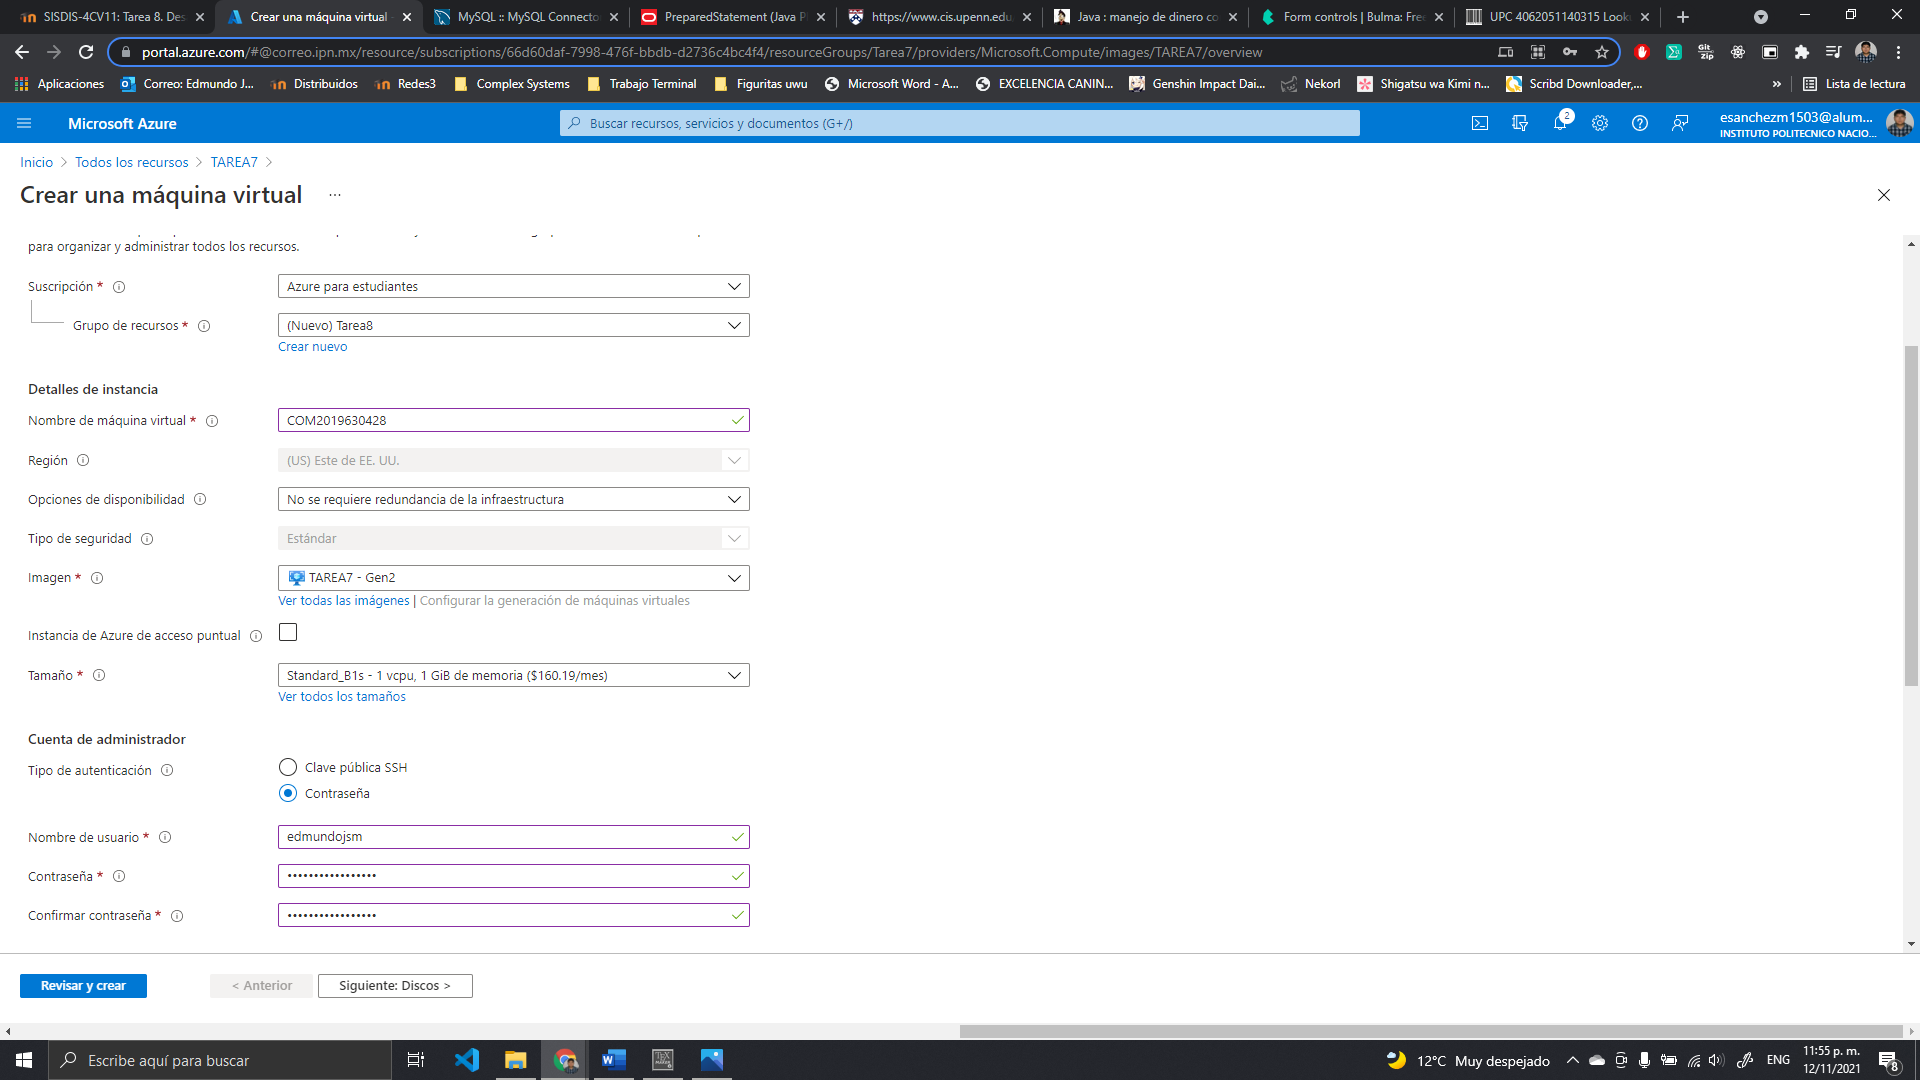
\includegraphics[scale=0.34]{resources/Infobasica.png}
			\caption{Datos básicos de la maquina virtual.}\label{fig:picture}
		\end{figure}
		\begin{figure}[H]
			\centering
			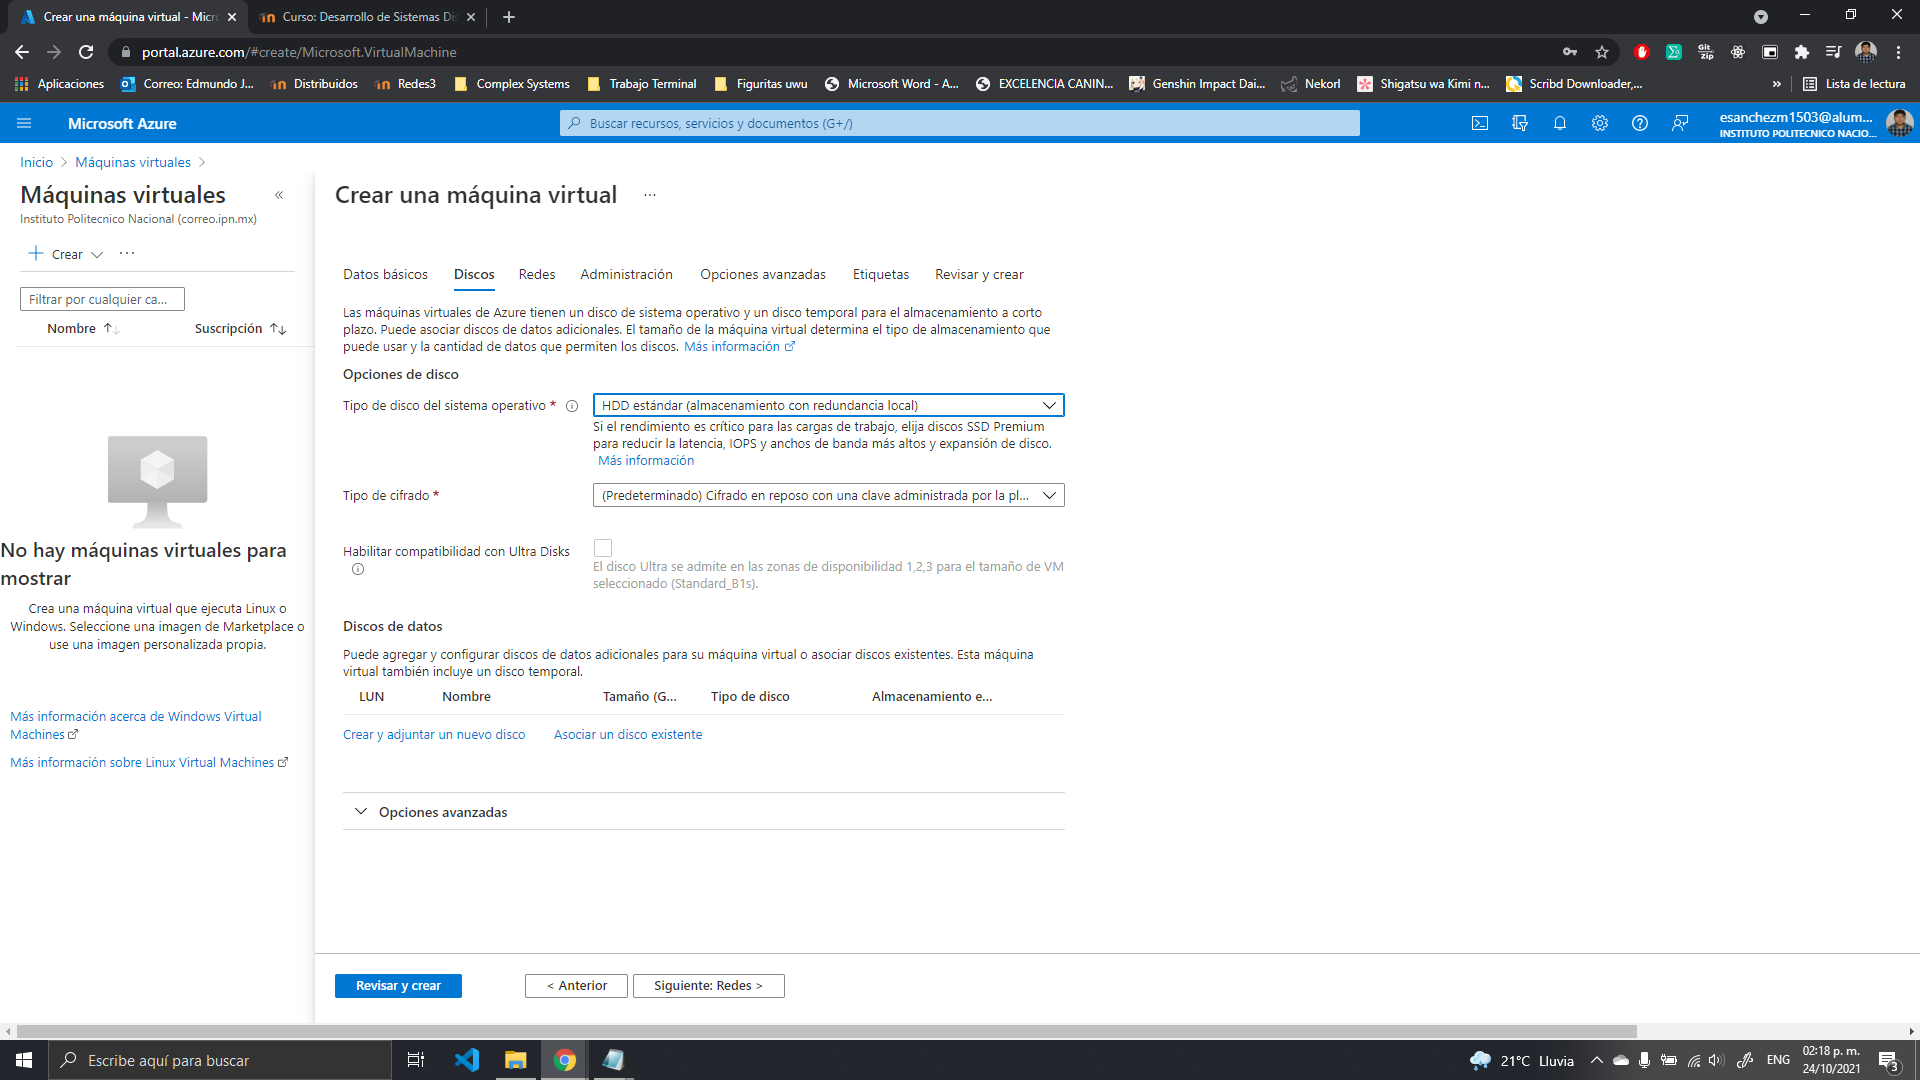
\includegraphics[scale=0.34]{resources/disco.png}
			\caption{Configuración del tipo de disco de la maquina virtual.}\label{fig:picture}
		\end{figure}
		\begin{figure}[H]
			\centering
			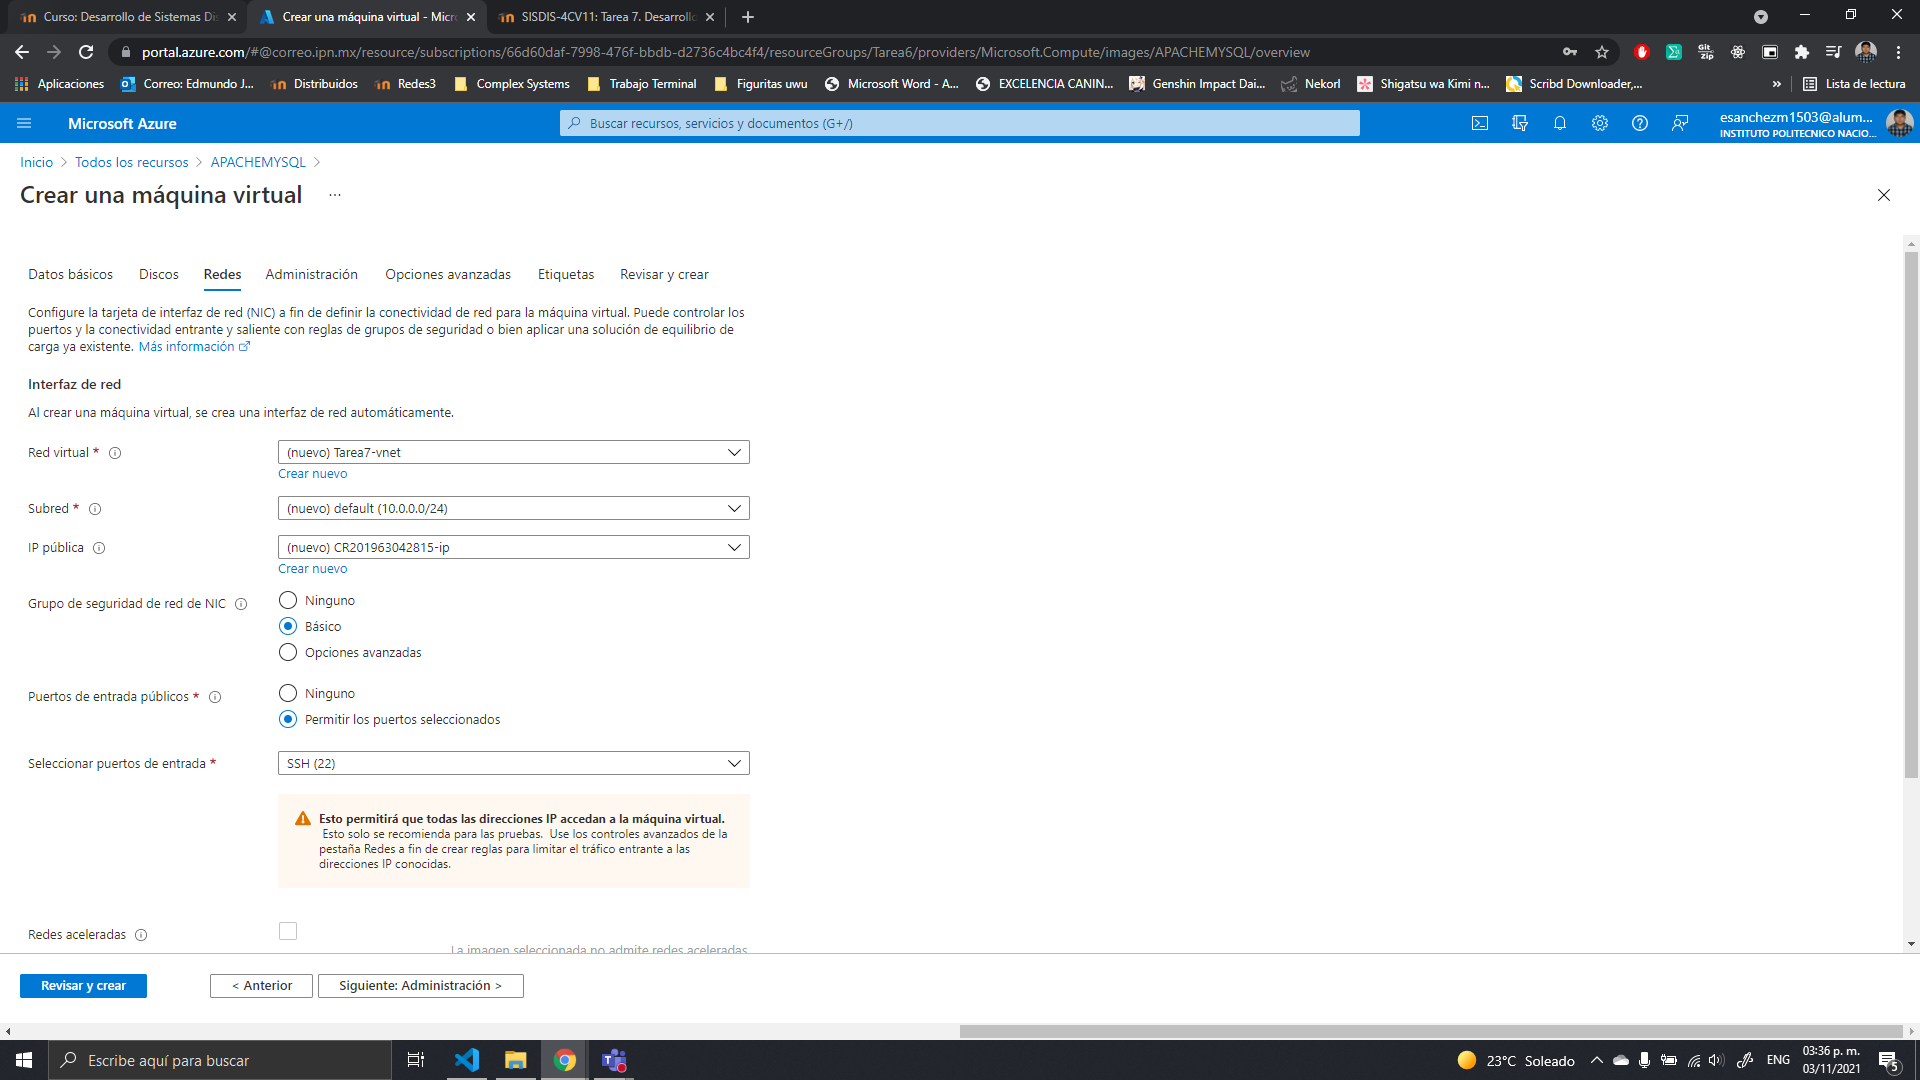
\includegraphics[scale=0.34]{resources/redes.png}
			\caption{Información sobre la redes de la maquina virtual.}\label{fig:picture}
		\end{figure}
		\begin{figure}[H]
			\centering
			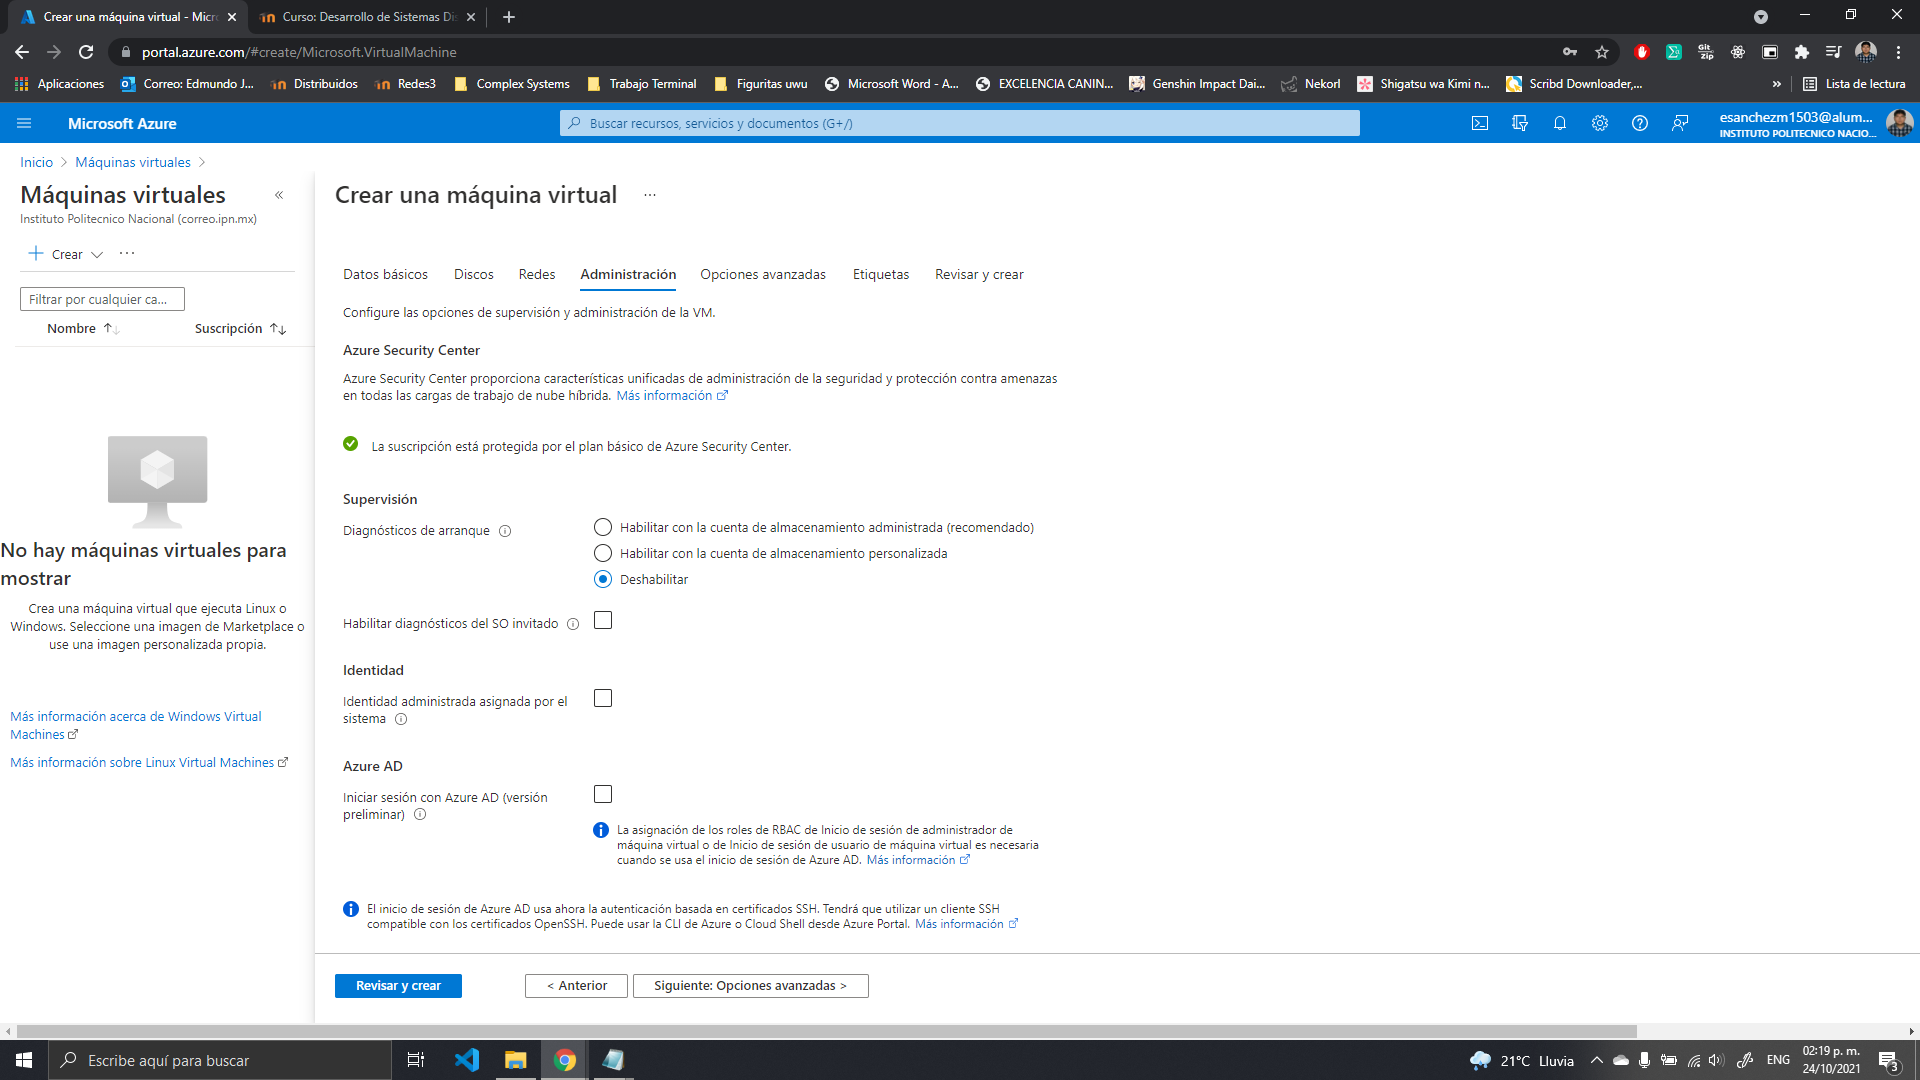
\includegraphics[scale=0.34]{resources/admin.png}
			\caption{Configuración de la administración de la maquina virtual.}\label{fig:picture}
		\end{figure}
		\begin{figure}[H]
			\centering
			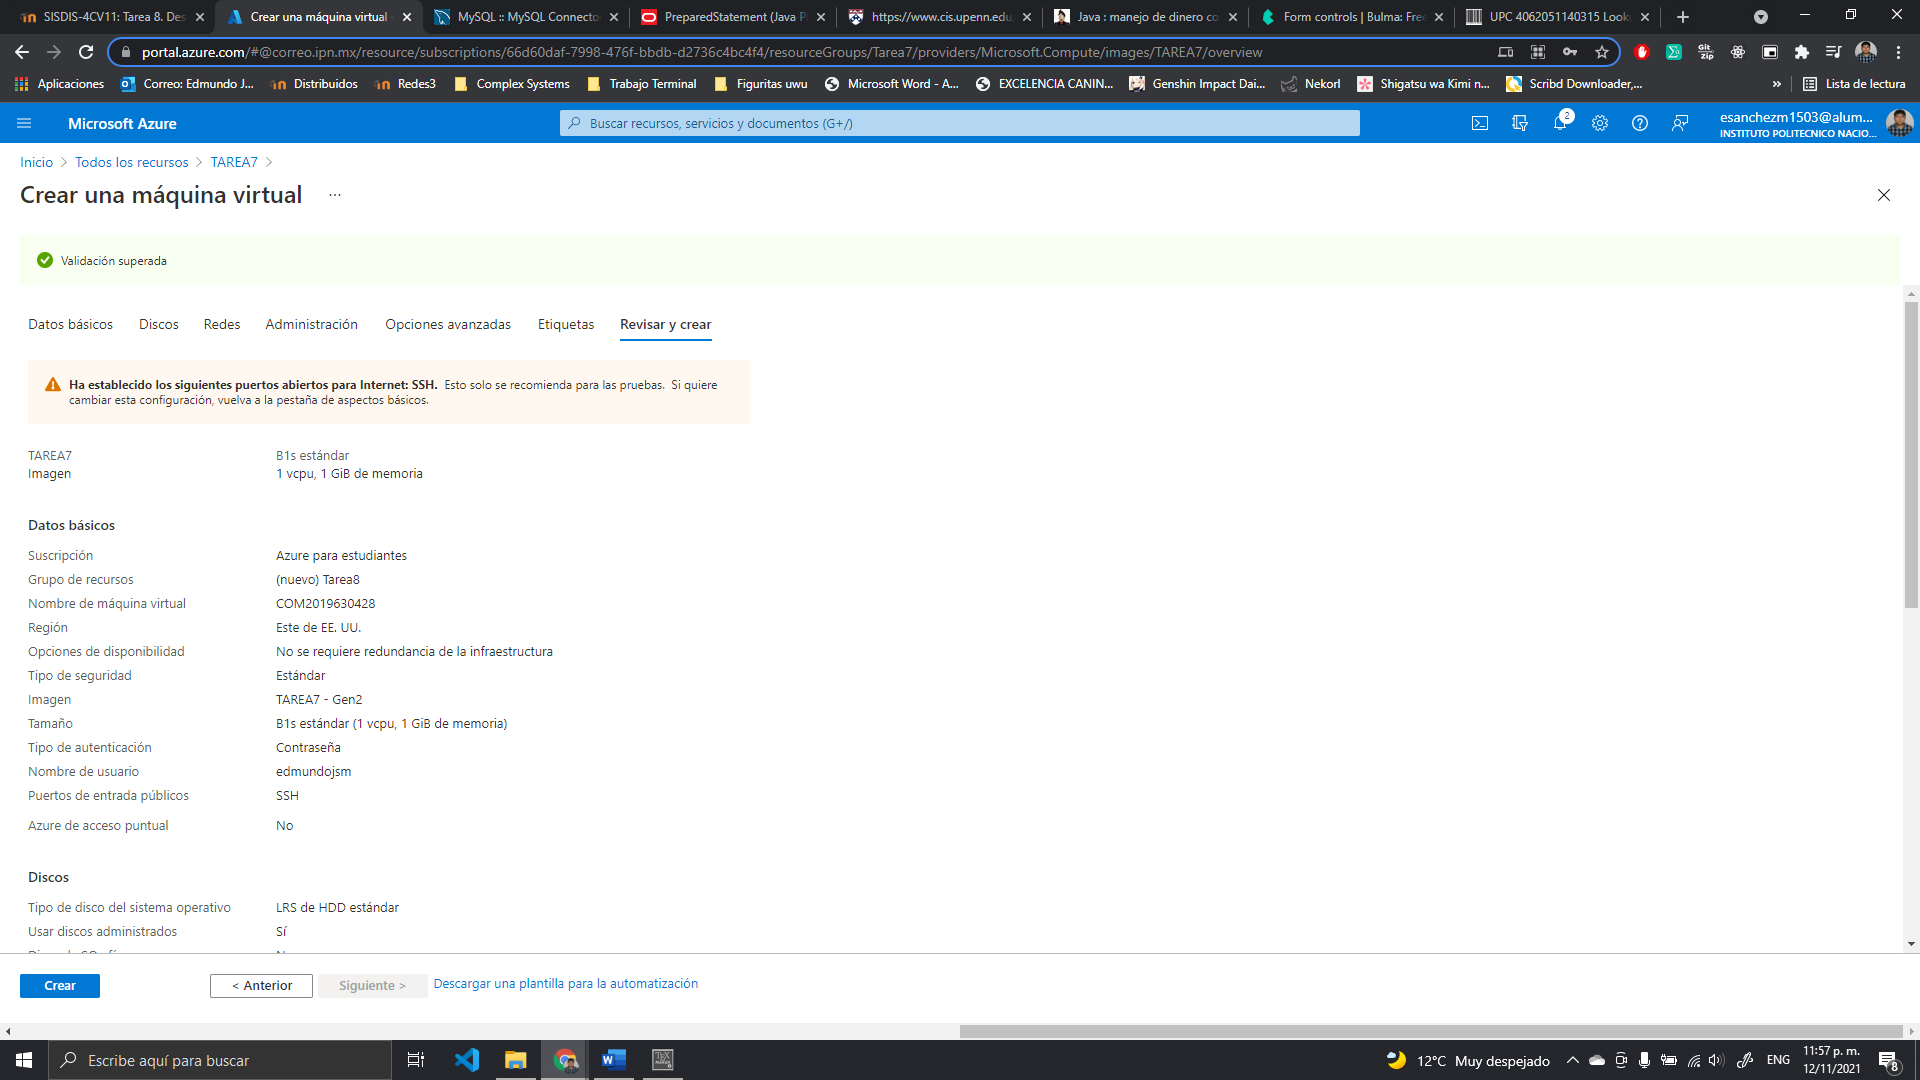
\includegraphics[scale=0.34]{resources/revisarycrear.png}
			\caption{Creación de la maquina virtual.}\label{fig:picture}
		\end{figure}
		\begin{figure}[H]
			\centering
			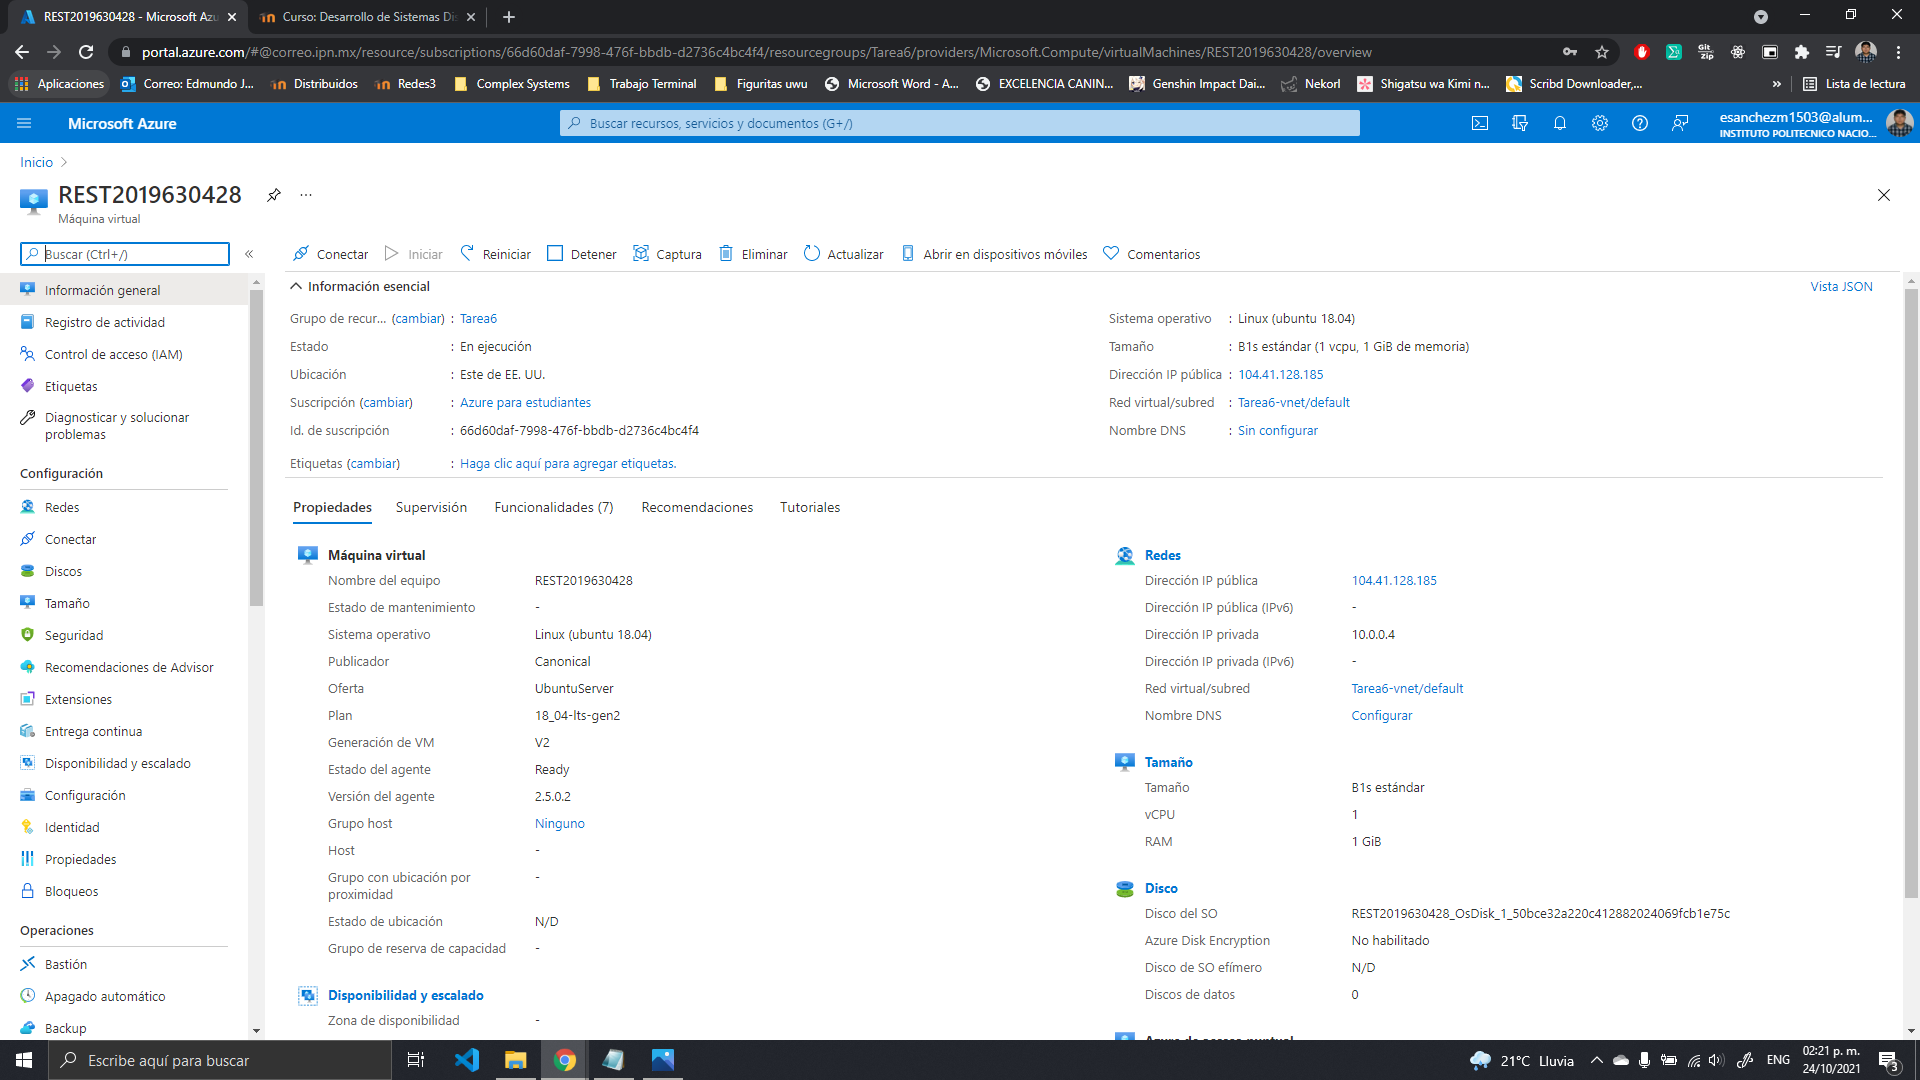
\includegraphics[scale=0.34]{resources/paneldecontrol.png}
			\caption{Panel de control de la maquina virtual.}\label{fig:picture}
		\end{figure}
		Una vez creada la maquina virtual tenemos que abrir el puerto 8080, ya que este puerto es el que ocupa Apache Tomcat, así podemos conectarnos de manera remota desde cualquier dispositivo , también es importante mencionar que si no se configura de manera correcta el puerto 8080 la conexión con la maquina virtual para poder visualizar el servicio web. En las figuras 7 y 8 podemos ver la configuración del puerto.
		\begin{figure}[H]
			\centering
			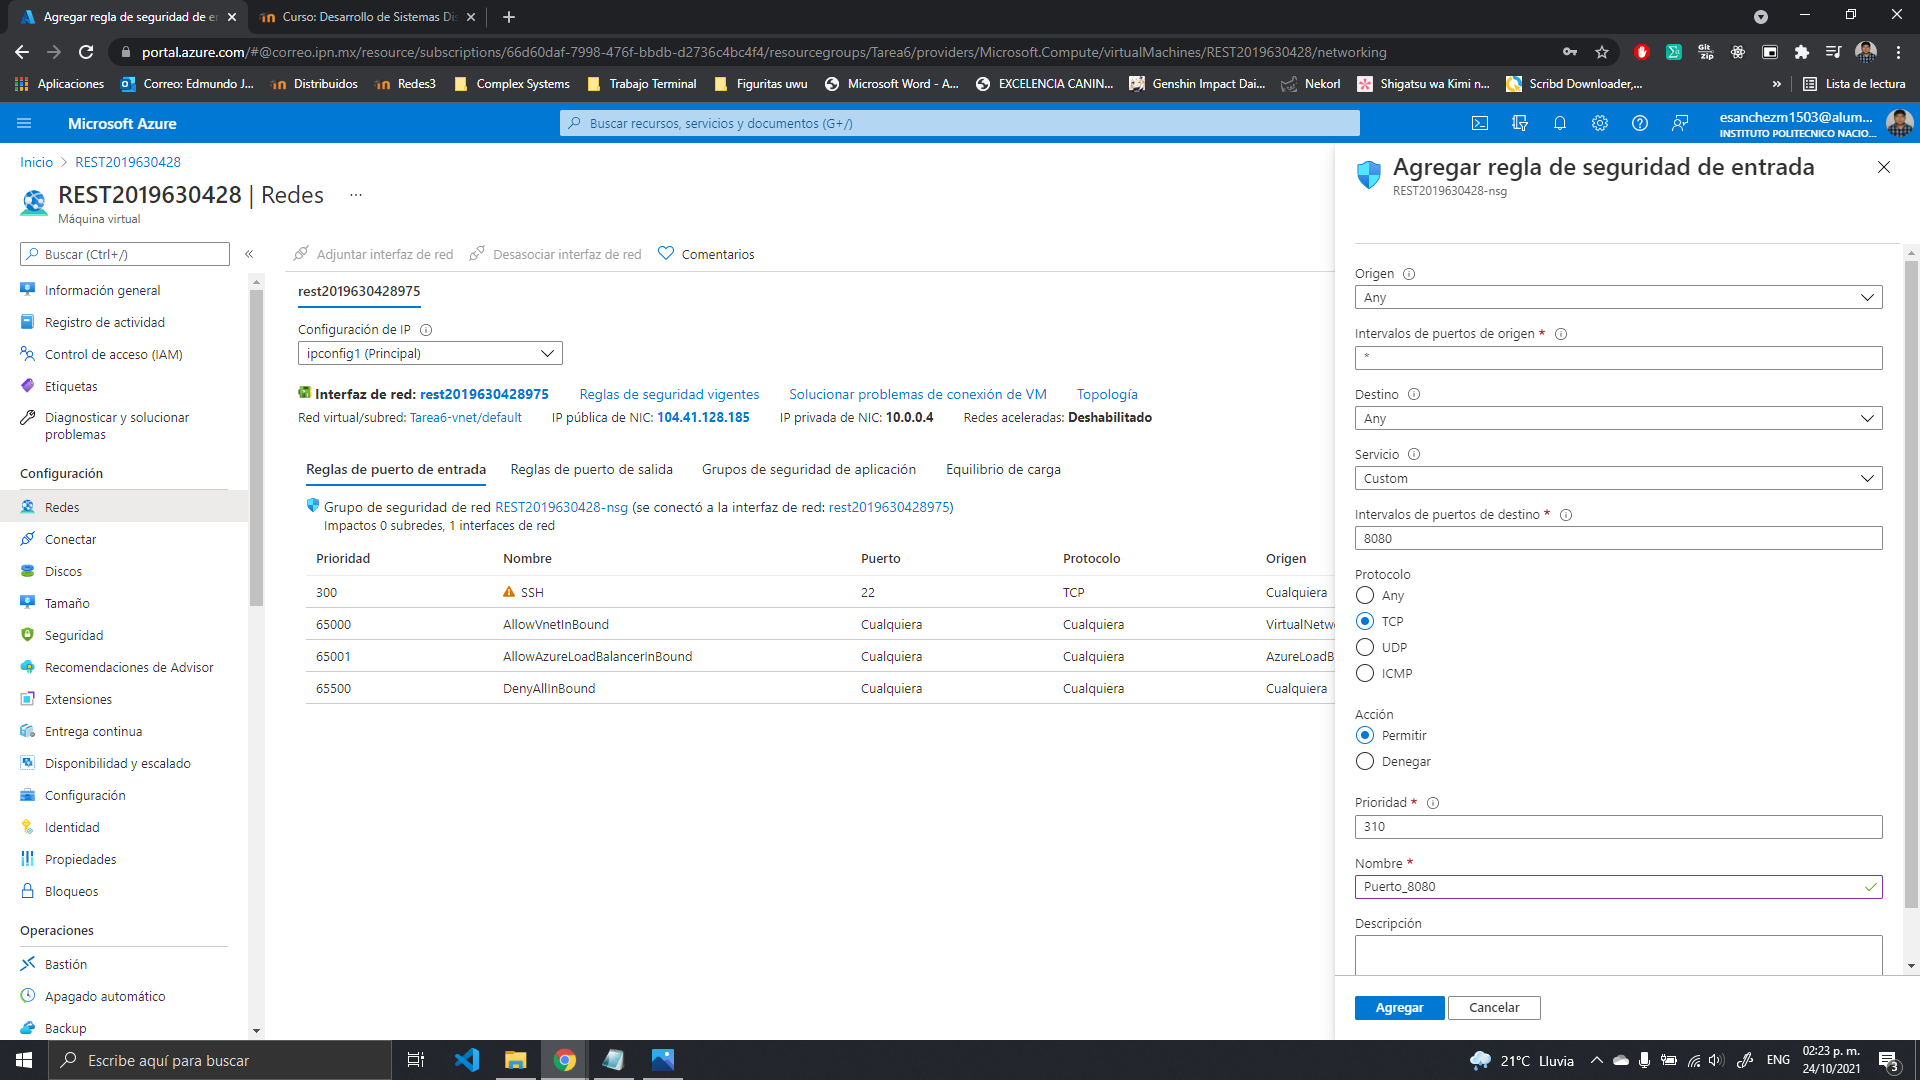
\includegraphics[scale=0.34]{resources/open8080.png}
			\caption{Configuración del puerto 8080.}\label{fig:picture}
		\end{figure}
		\begin{figure}[H]
			\centering
			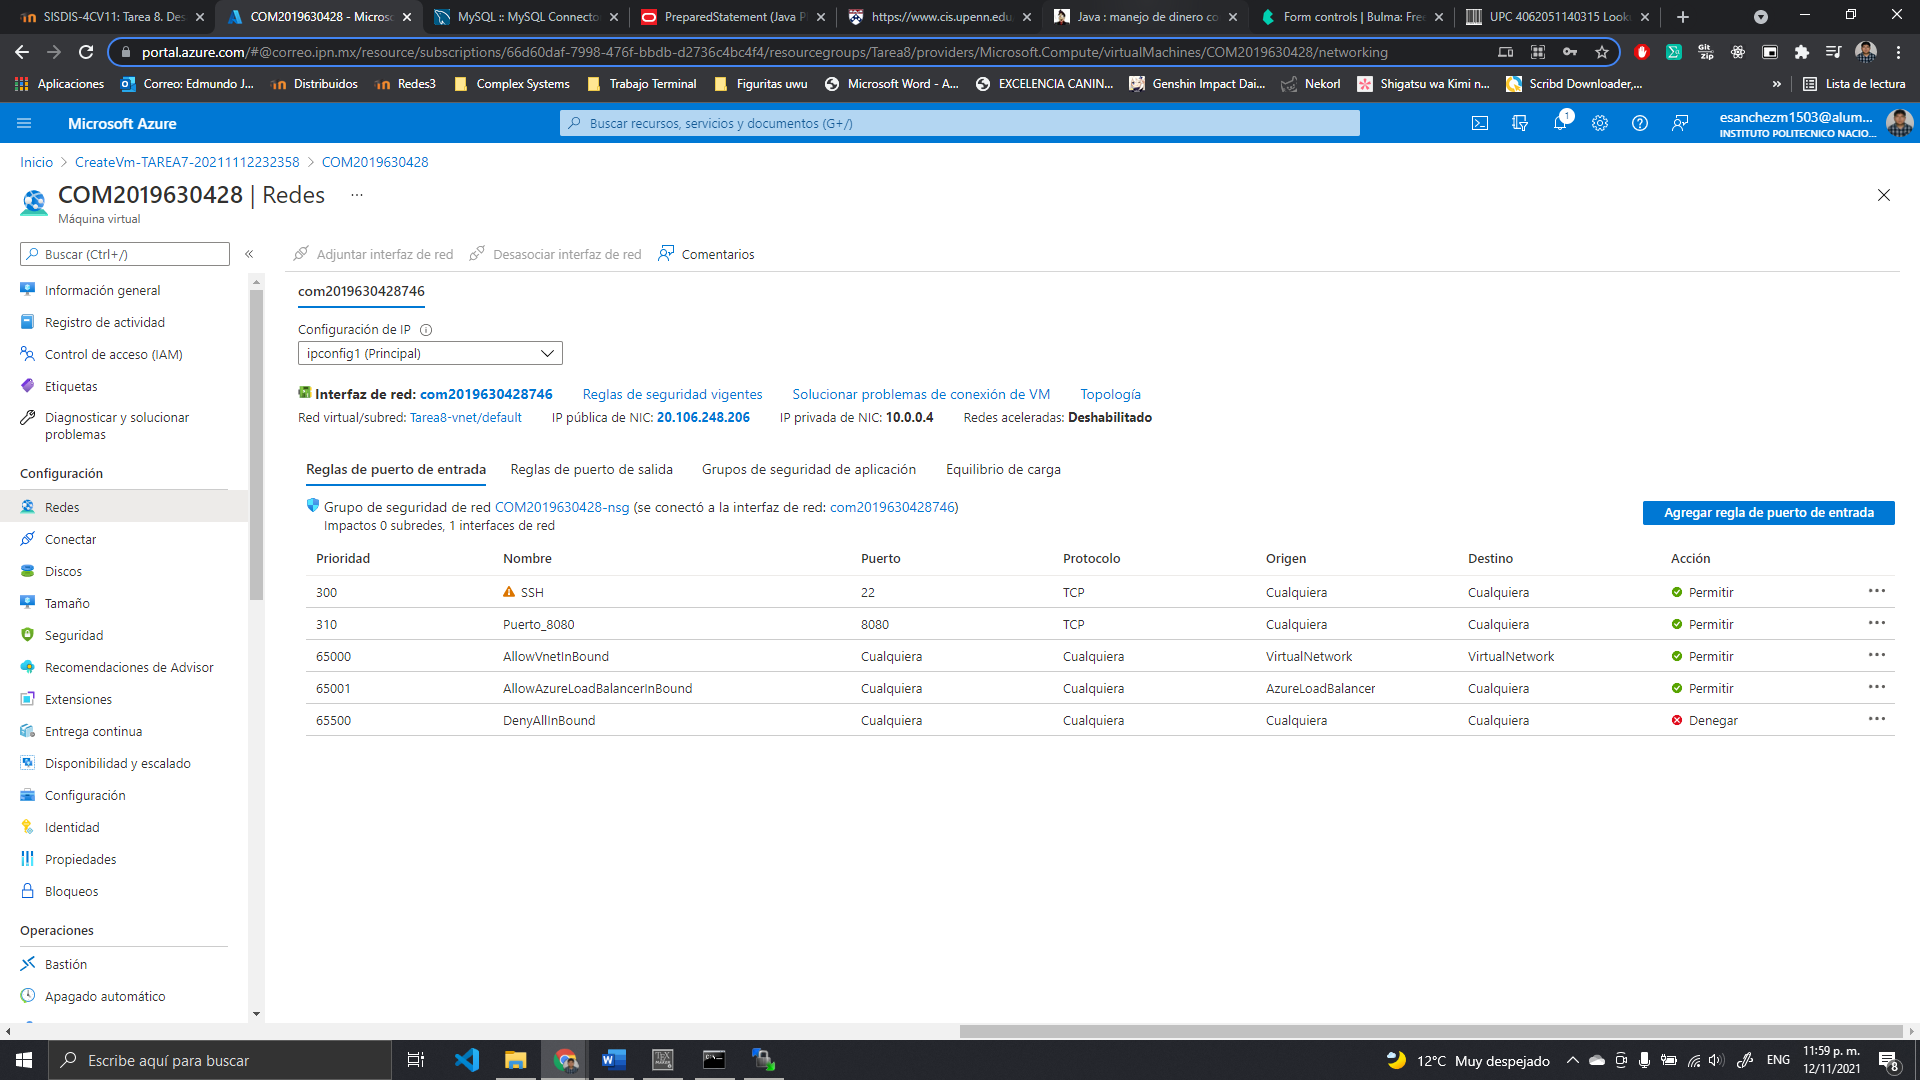
\includegraphics[scale=0.34]{resources/puertook.png}
			\caption{Puerto 8080 abierto correctamente.}\label{fig:picture}
		\end{figure}
		Ya teniendo la maquina preparada, procederemos a realizar los cambios en Servicio.java para poder cumplir con los requerimientos de la practica.
		\subsection{Cambios hechos en Servicio.java y Usuario.java}
		Primero que nada nos tendremos que conectar por medio de ssh a la maquina virtual como vemos en la figura 9.
		\begin{figure}[H]
			\centering
			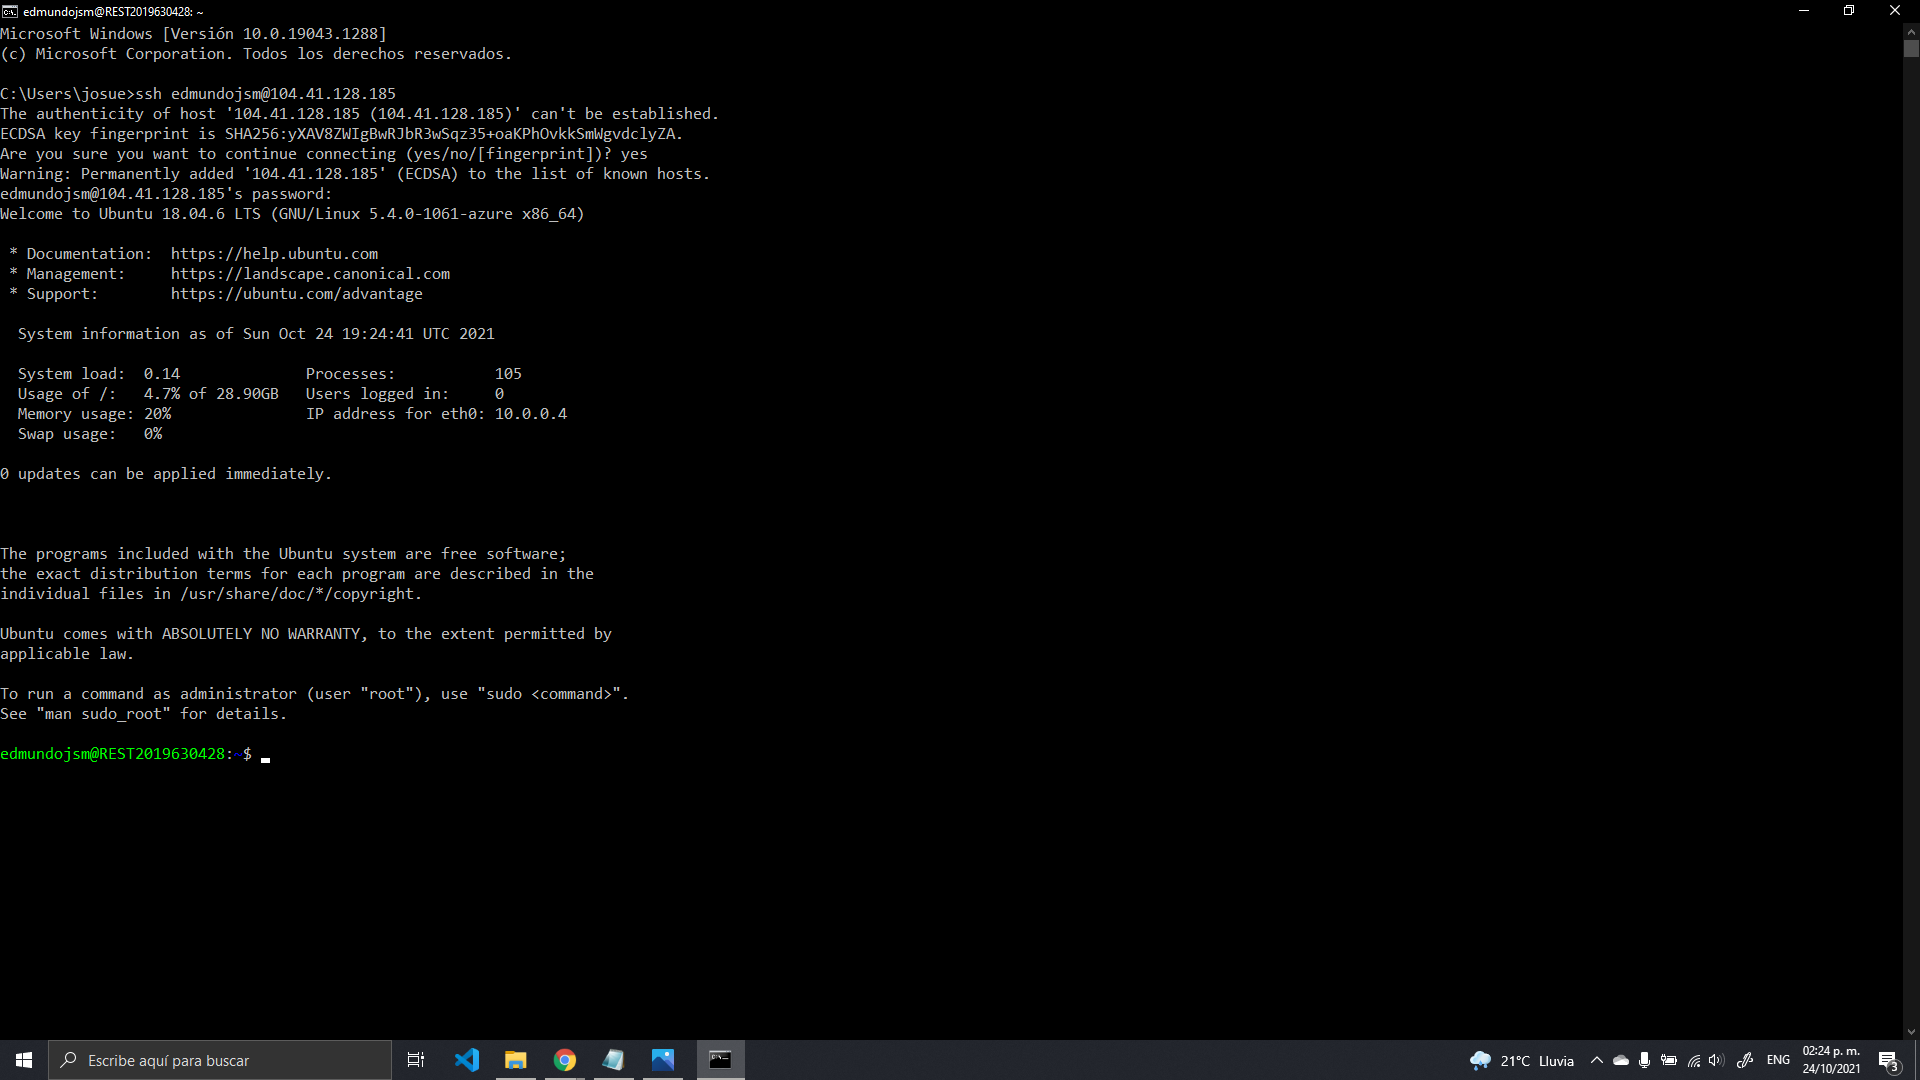
\includegraphics[scale=0.34]{resources/conexionssh.png}
			\caption{Conexión ssh con la maquina virtual.}\label{fig:picture}
		\end{figure}
		Posteriormente realizaremos los cambios correspondientes, en primer lugar vamos a agregar el campo id\_usuario a la clase Usuario.java como se ve en la figura 10.
		\begin{figure}[H]
			\centering
			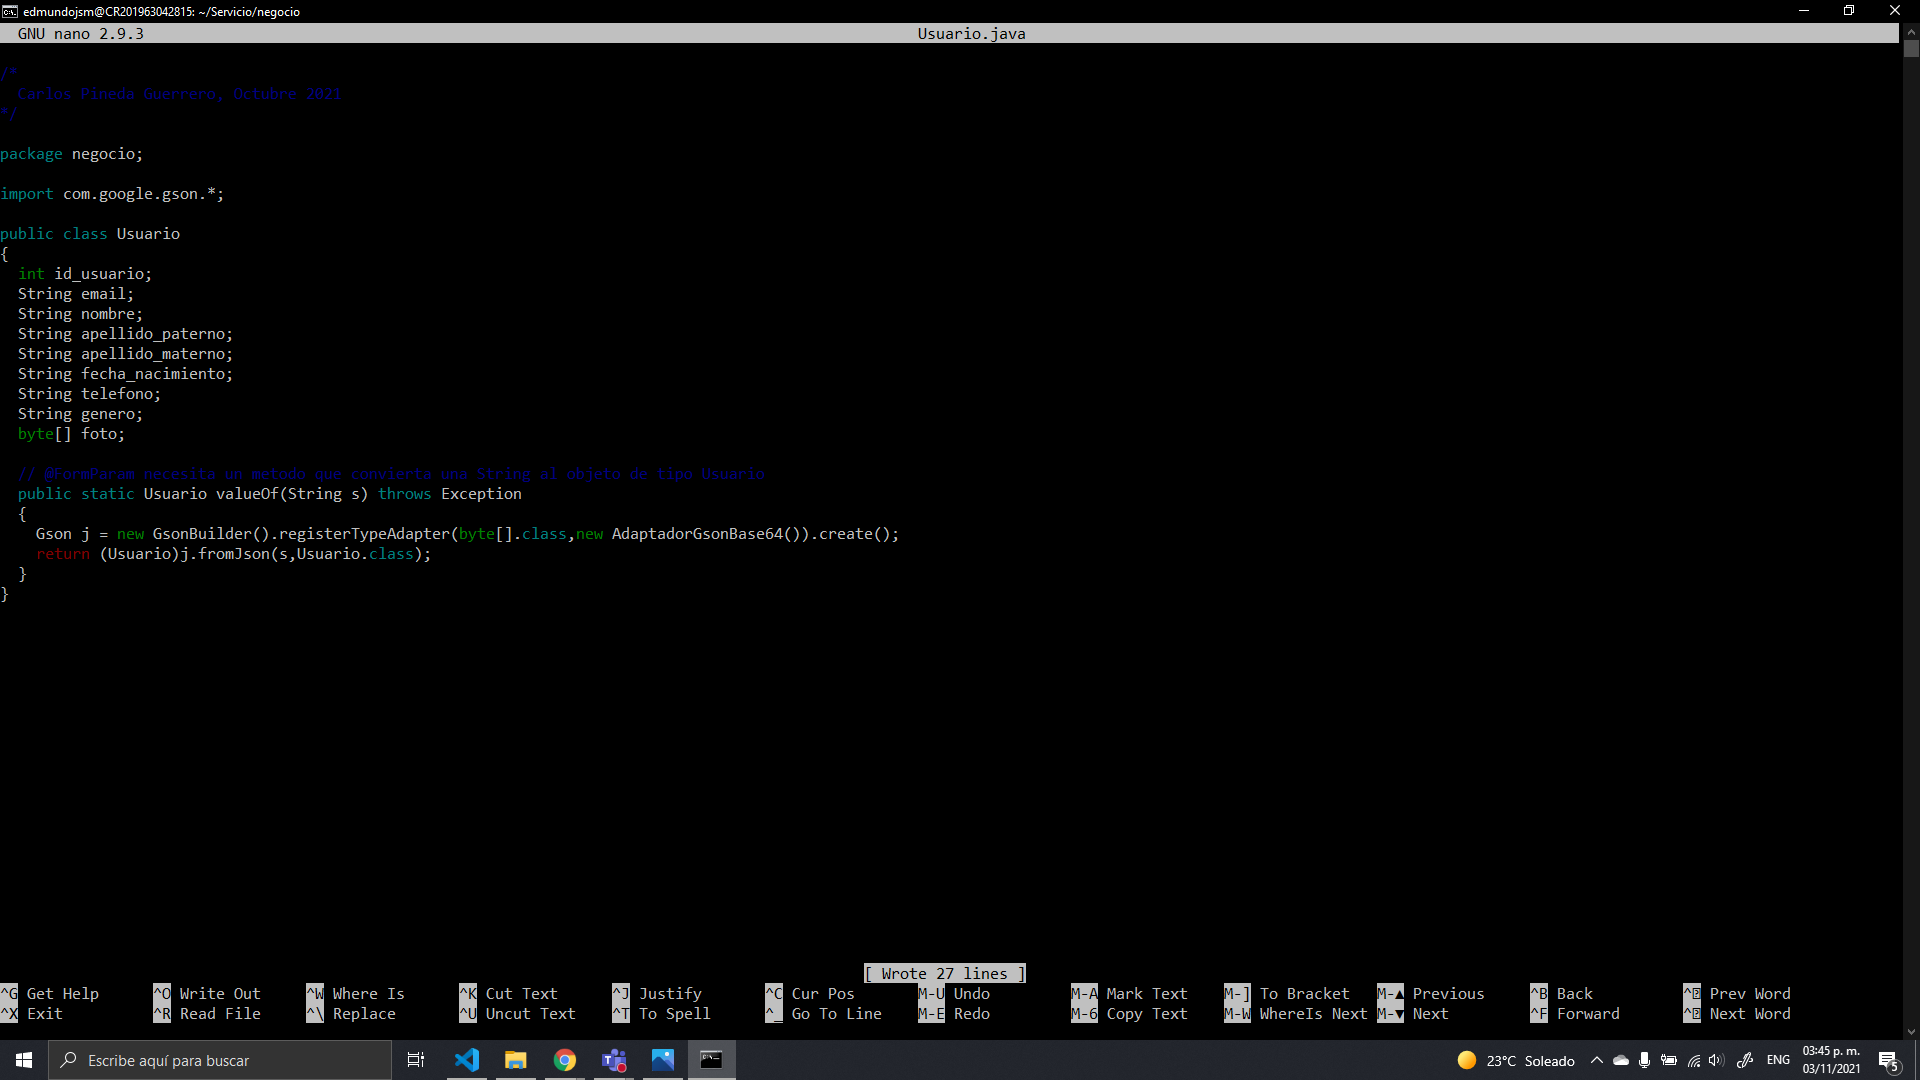
\includegraphics[scale=0.34]{resources/p1.png}
			\caption{Campo id\_usuario agregado a la clase Usuario.java.}\label{fig:picture}
		\end{figure}
		Ahora en las figuras 11 y 12 podemos ver las modificaciones necesarias para cumplir el punto 2 de las modificaciones solicitadas.
		\begin{figure}[H]
			\centering
			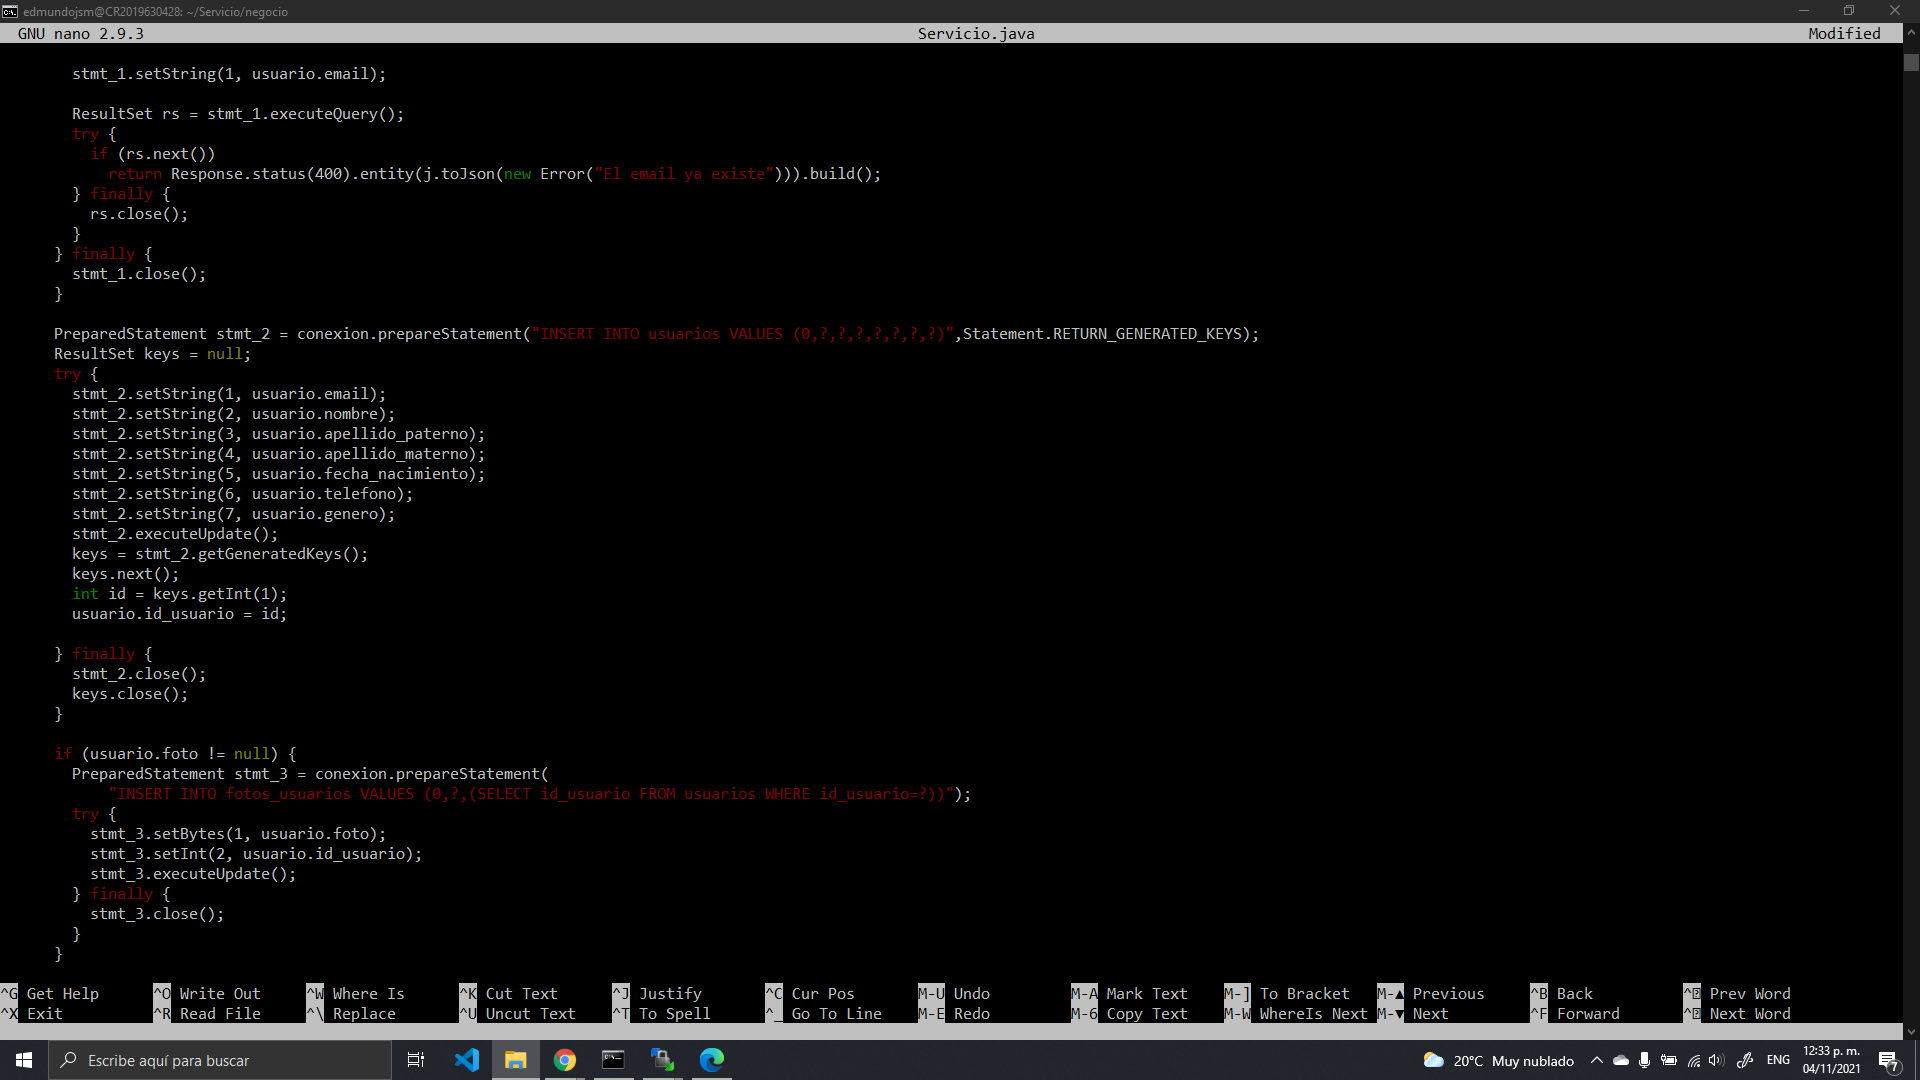
\includegraphics[scale=0.34]{resources/p2.png}
			\caption{Cambios para cumplir el punto 2 de las modificaciones solicitadas. Parte 1.}	\label{fig:picture}
		\end{figure}
		\begin{figure}[H]
			\centering
			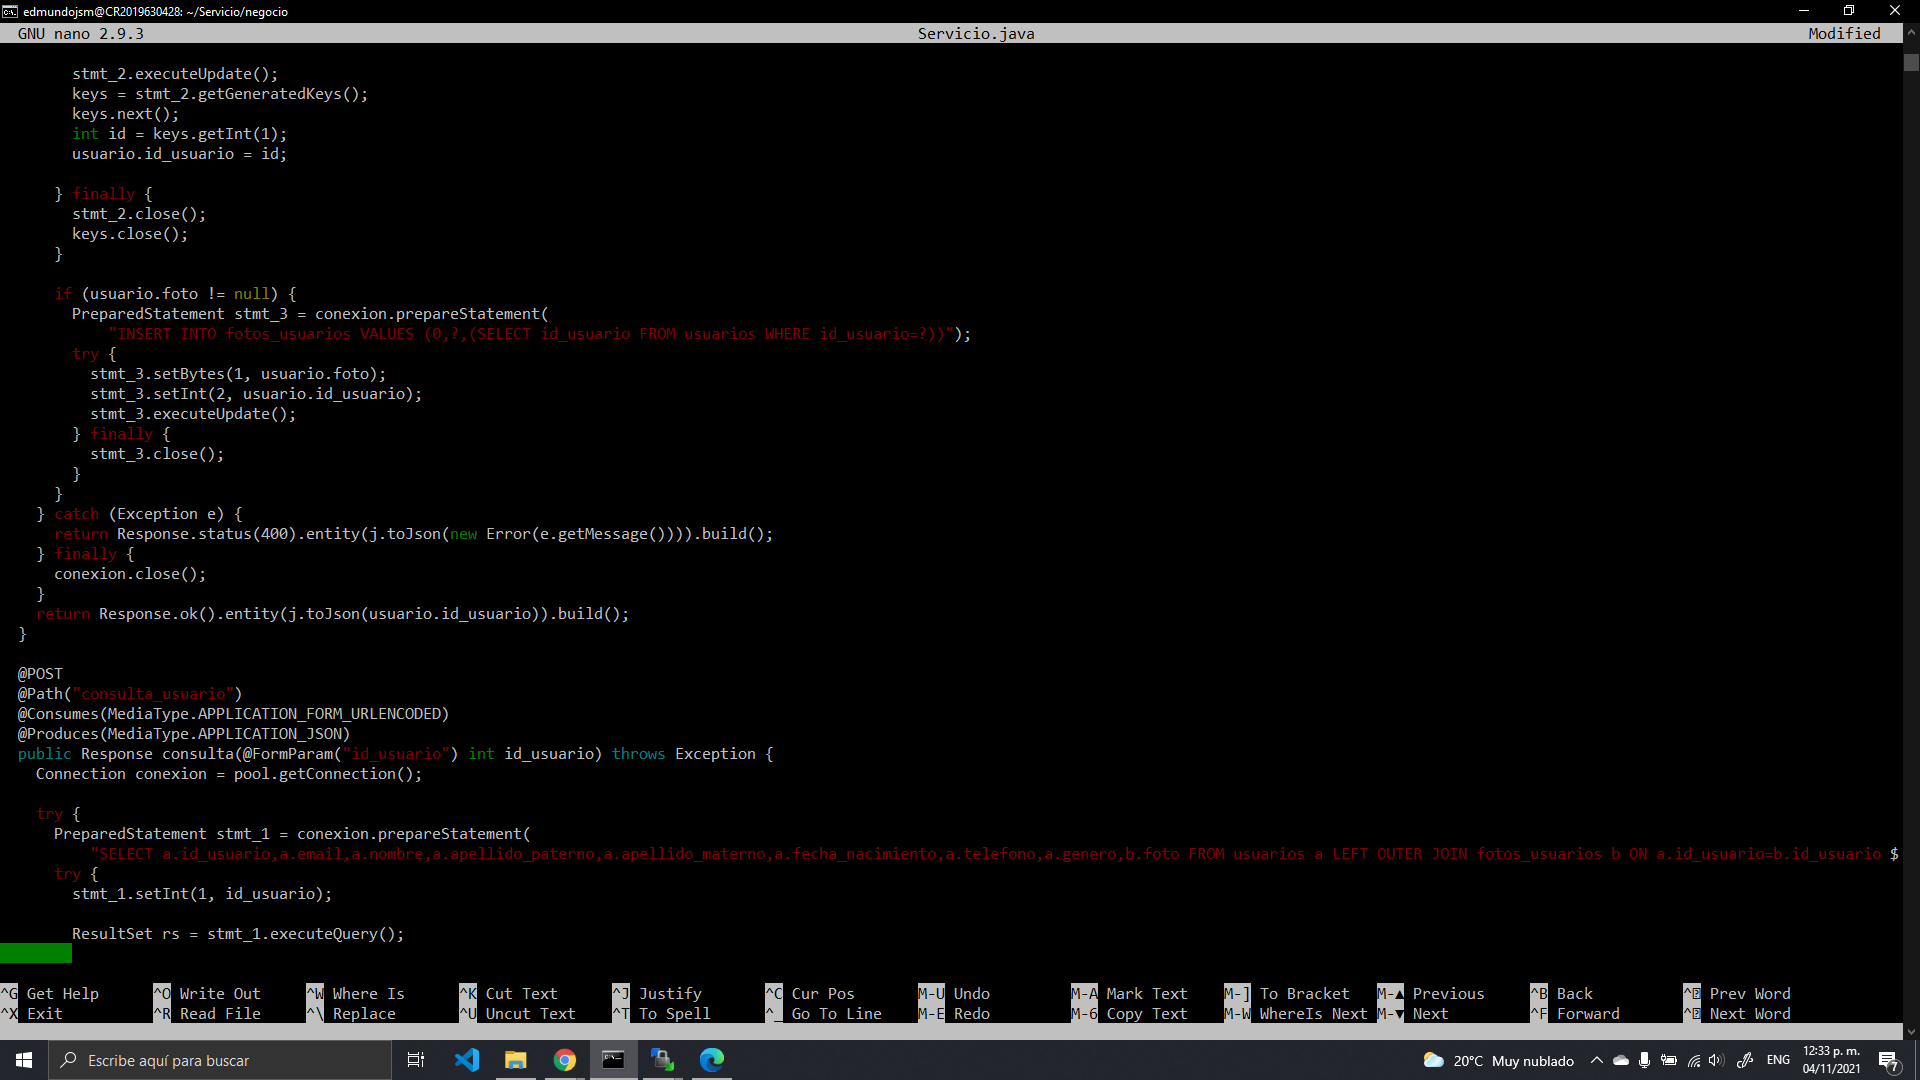
\includegraphics[scale=0.34]{resources/p2.1p3.png}
			\caption{Cambios para cumplir el punto 2 de las modificaciones solicitadas. Parte 2.}	\label{fig:picture}
		\end{figure}
		Después llevamos acabo lo solicitado en el punto 3, esto lo podemos ver en la figura 12 al final cuando ponemos como parámetro el id del usuario y en la figura 13.
		\begin{figure}[H]
			\centering
			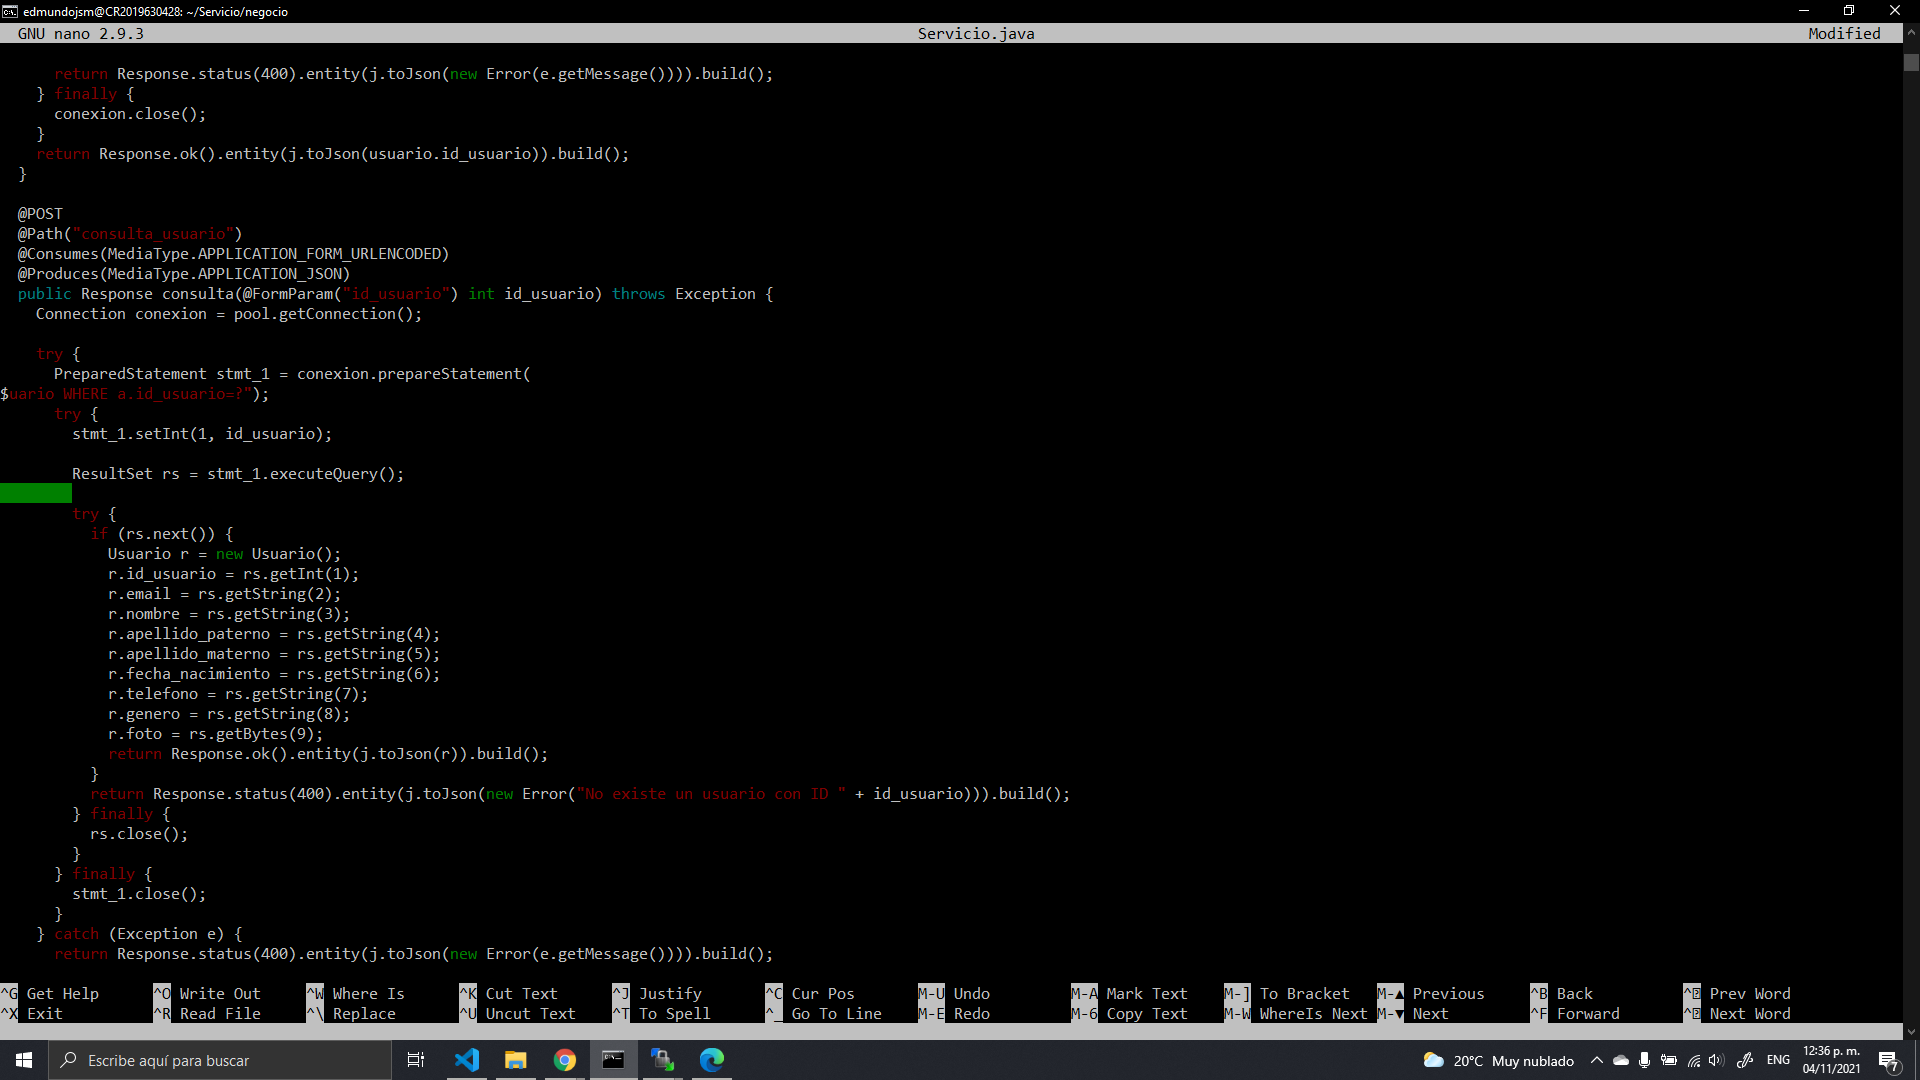
\includegraphics[scale=0.34]{resources/p3.1.png}
			\caption{Cambios para cumplir el punto 3 de las modificaciones solicitadas.}\label{fig:picture}
		\end{figure}
		Después pasamos a cumplir el punto 4 como vemos en las figuras 14 y 15.
		\begin{figure}[H]
			\centering
			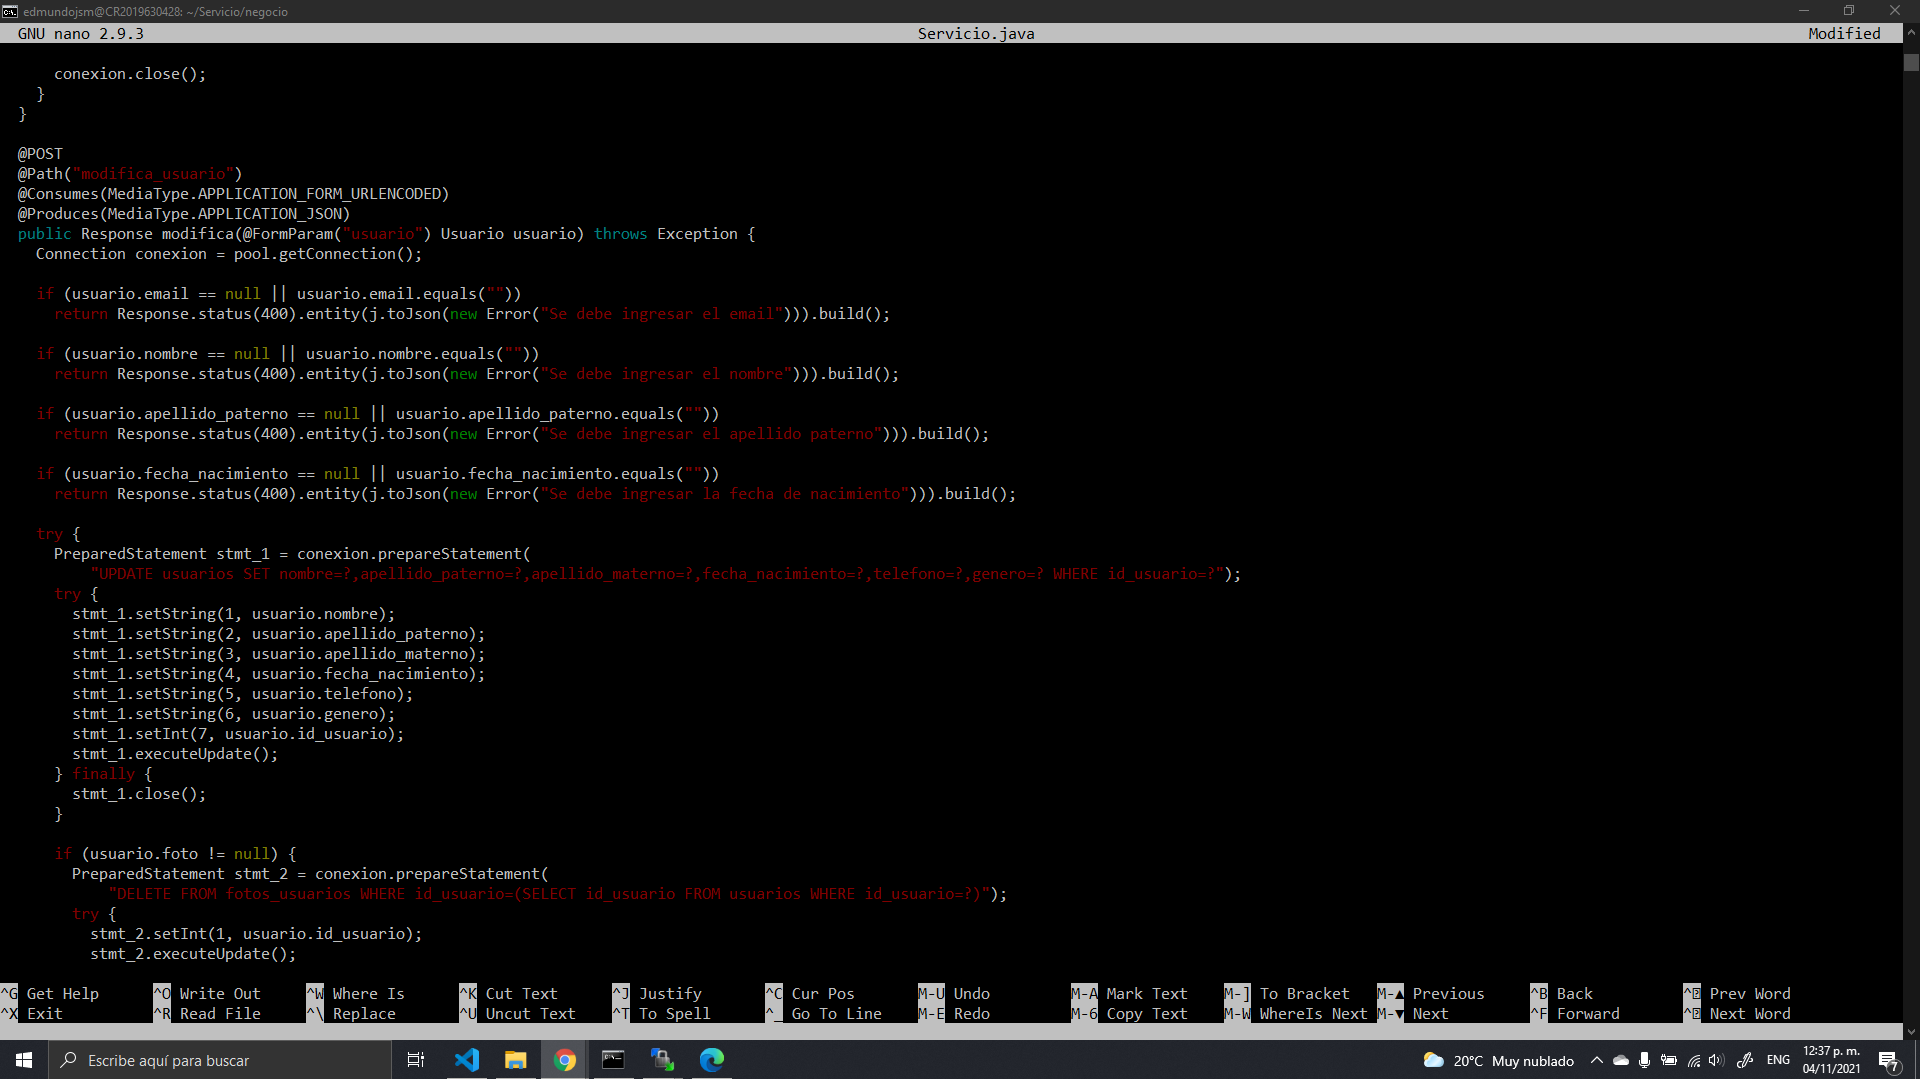
\includegraphics[scale=0.34]{resources/p4.png}
			\caption{Cambios para cumplir el punto 4 de las modificaciones solicitadas. Parte 1.}\label{fig:picture}
		\end{figure}
		\begin{figure}[H]
			\centering
			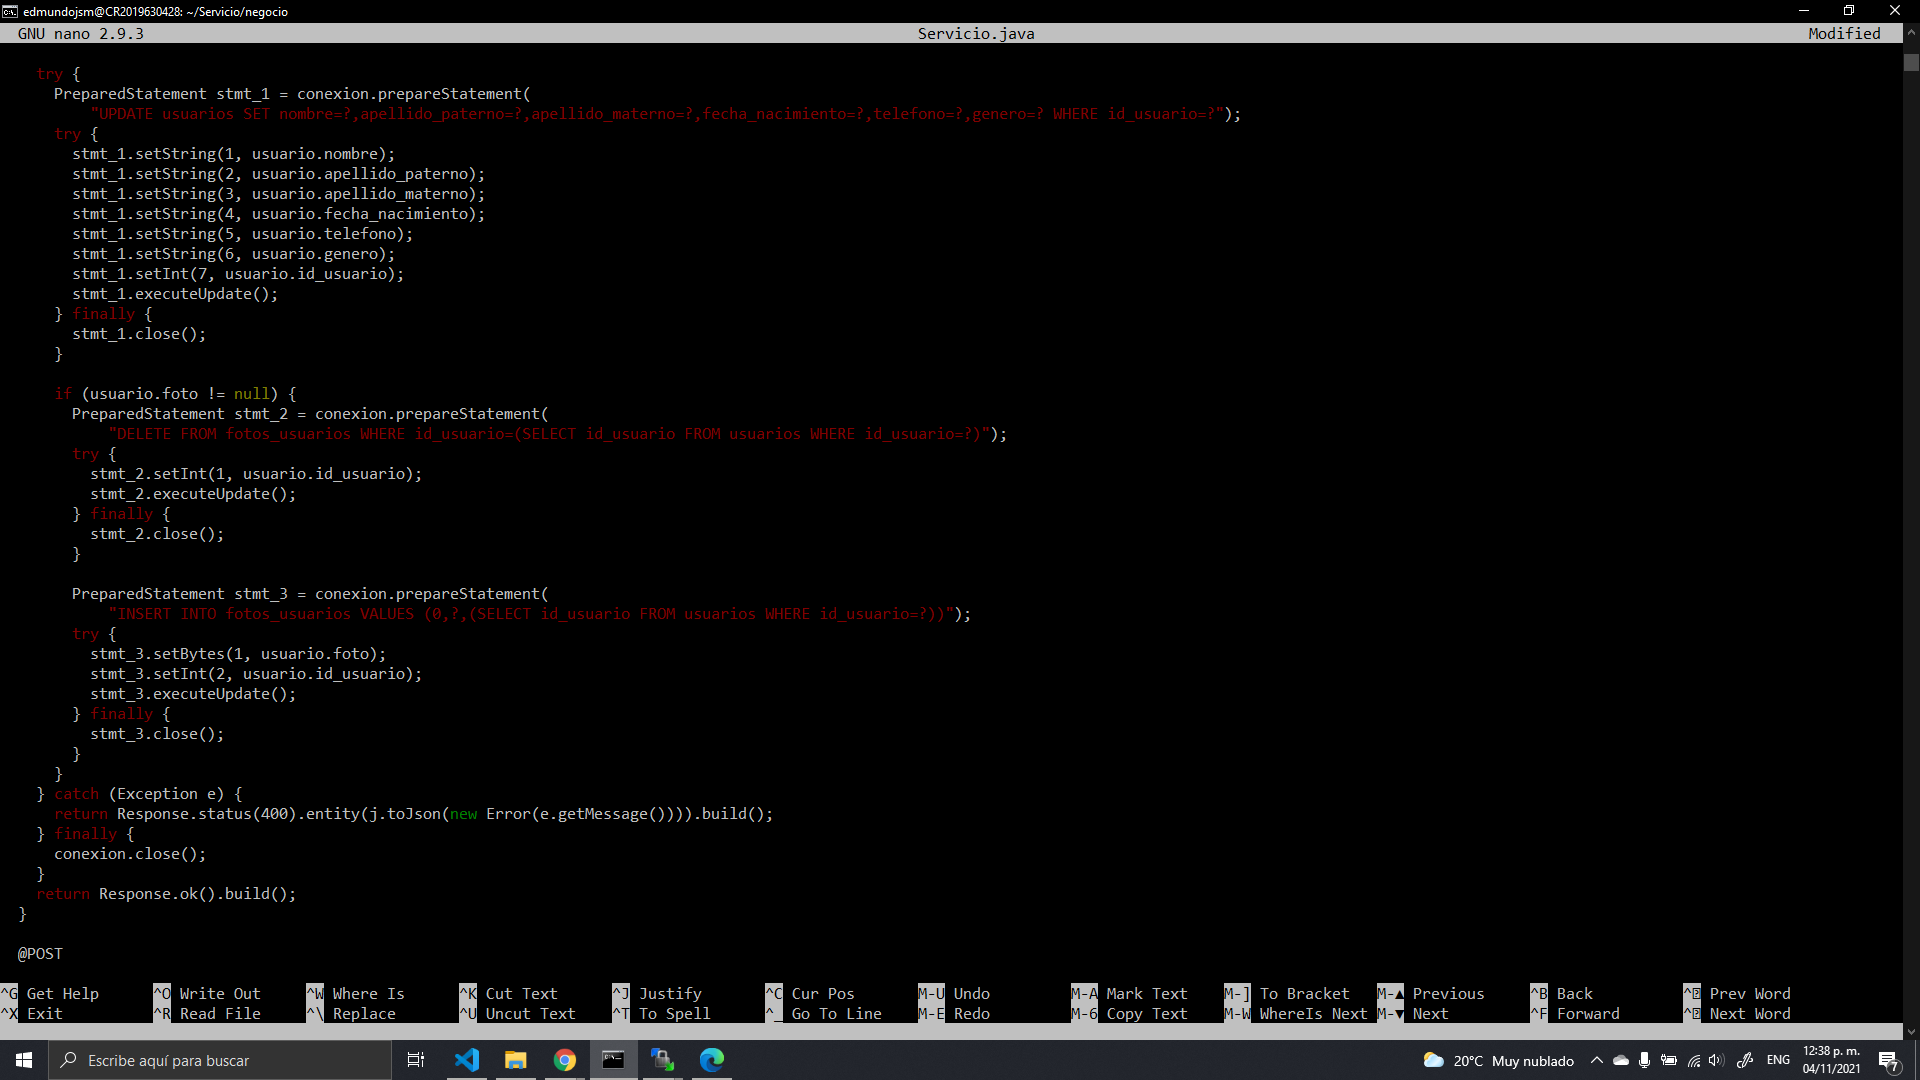
\includegraphics[scale=0.34]{resources/p4.1.png}
			\caption{Cambios para cumplir el punto 4 de las modificaciones solicitadas. Parte 2.}\label{fig:picture}
		\end{figure}
		Finalmente en la figura 16 podemos ver la modificación que se realizo para cumplir la ultima  solicitada.
		\begin{figure}[H]
			\centering
			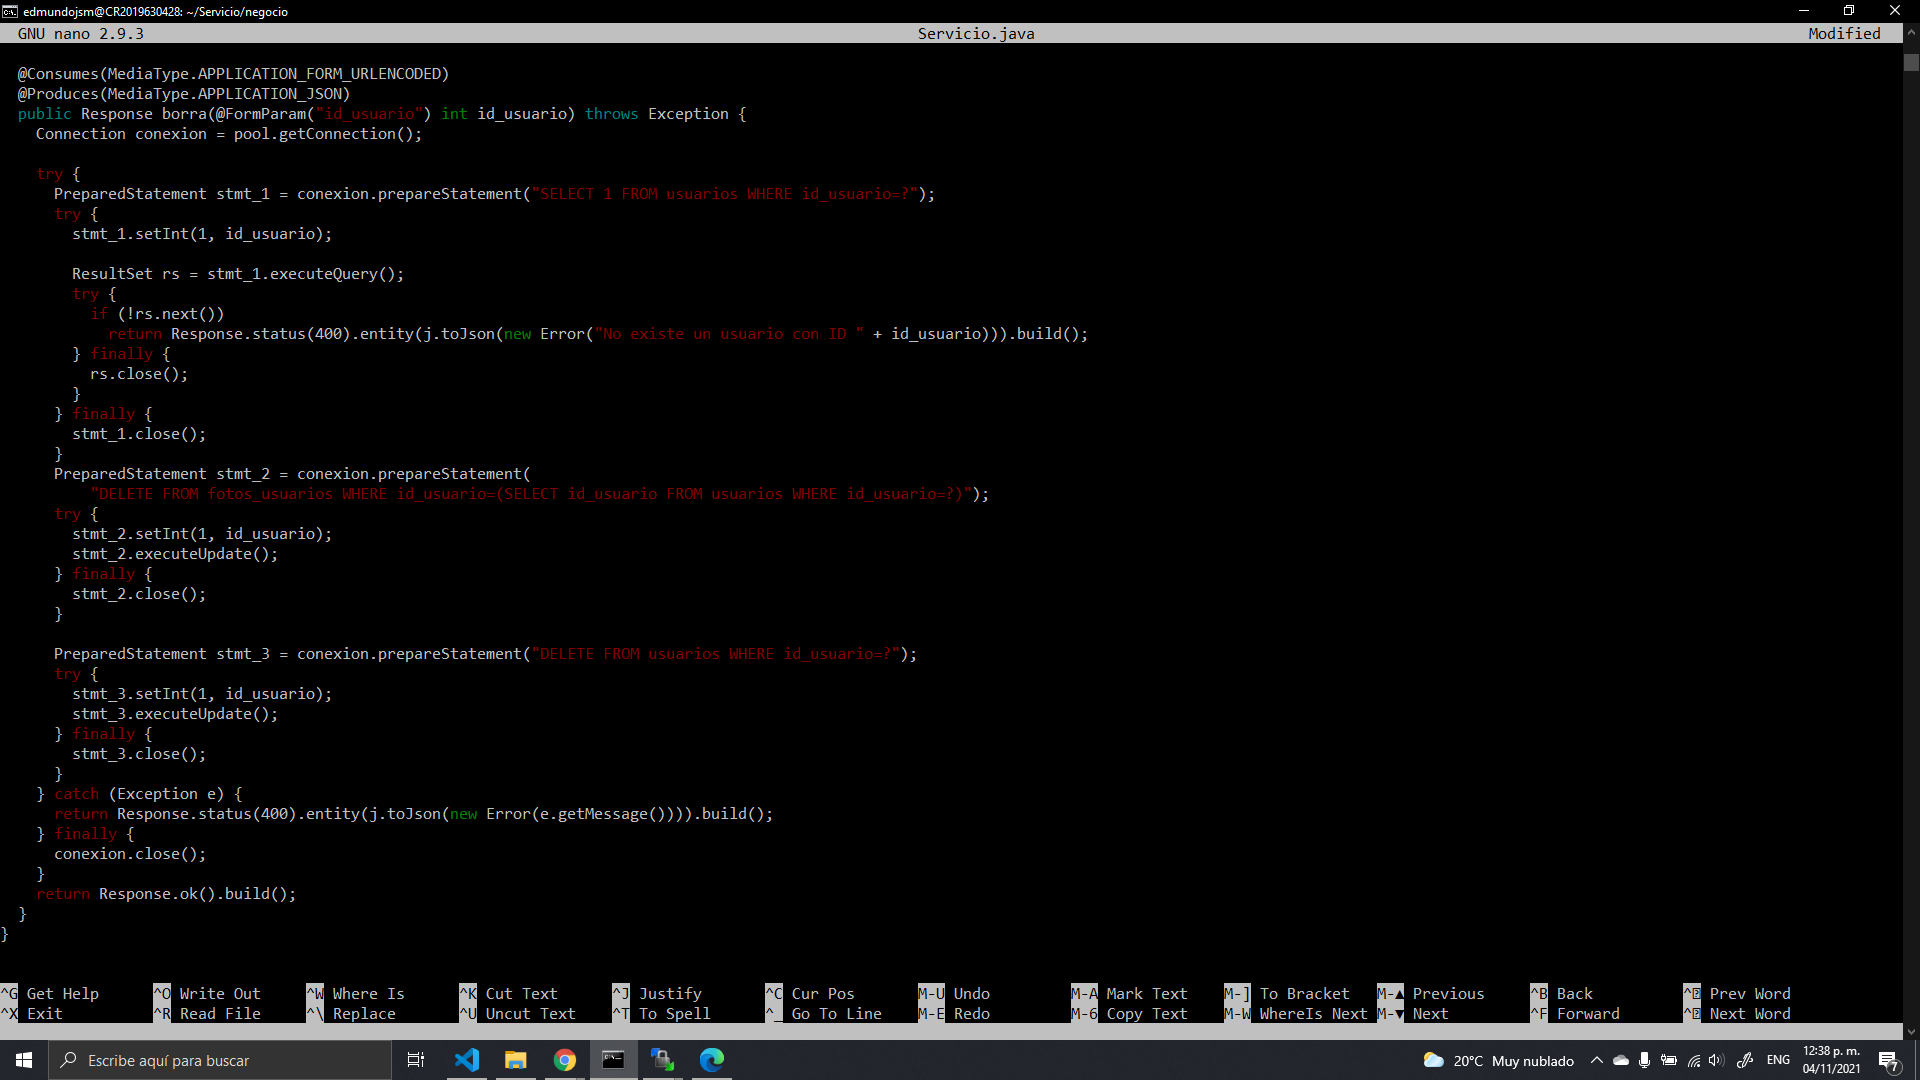
\includegraphics[scale=0.34]{resources/p5.png}
			\caption{Cambios para cumplir el punto 4 de las modificaciones solicitadas. Parte 2.}\label{fig:picture}
		\end{figure}
	\subsection{Preparación del entorno tanto en servidor como en el cliente}		
	Para empezar debemos de borrar el anterior Servicio de webapps ya que tenemos una actualización, esto lo podemos ver en la figura 17, después nos toca volver a configurar las variables de entorno de java jdk y CATALINA\_HOME y por supuesto correr Tomcat, esto se puede ver en la figura 18.
	\begin{figure}[H]
			\centering
			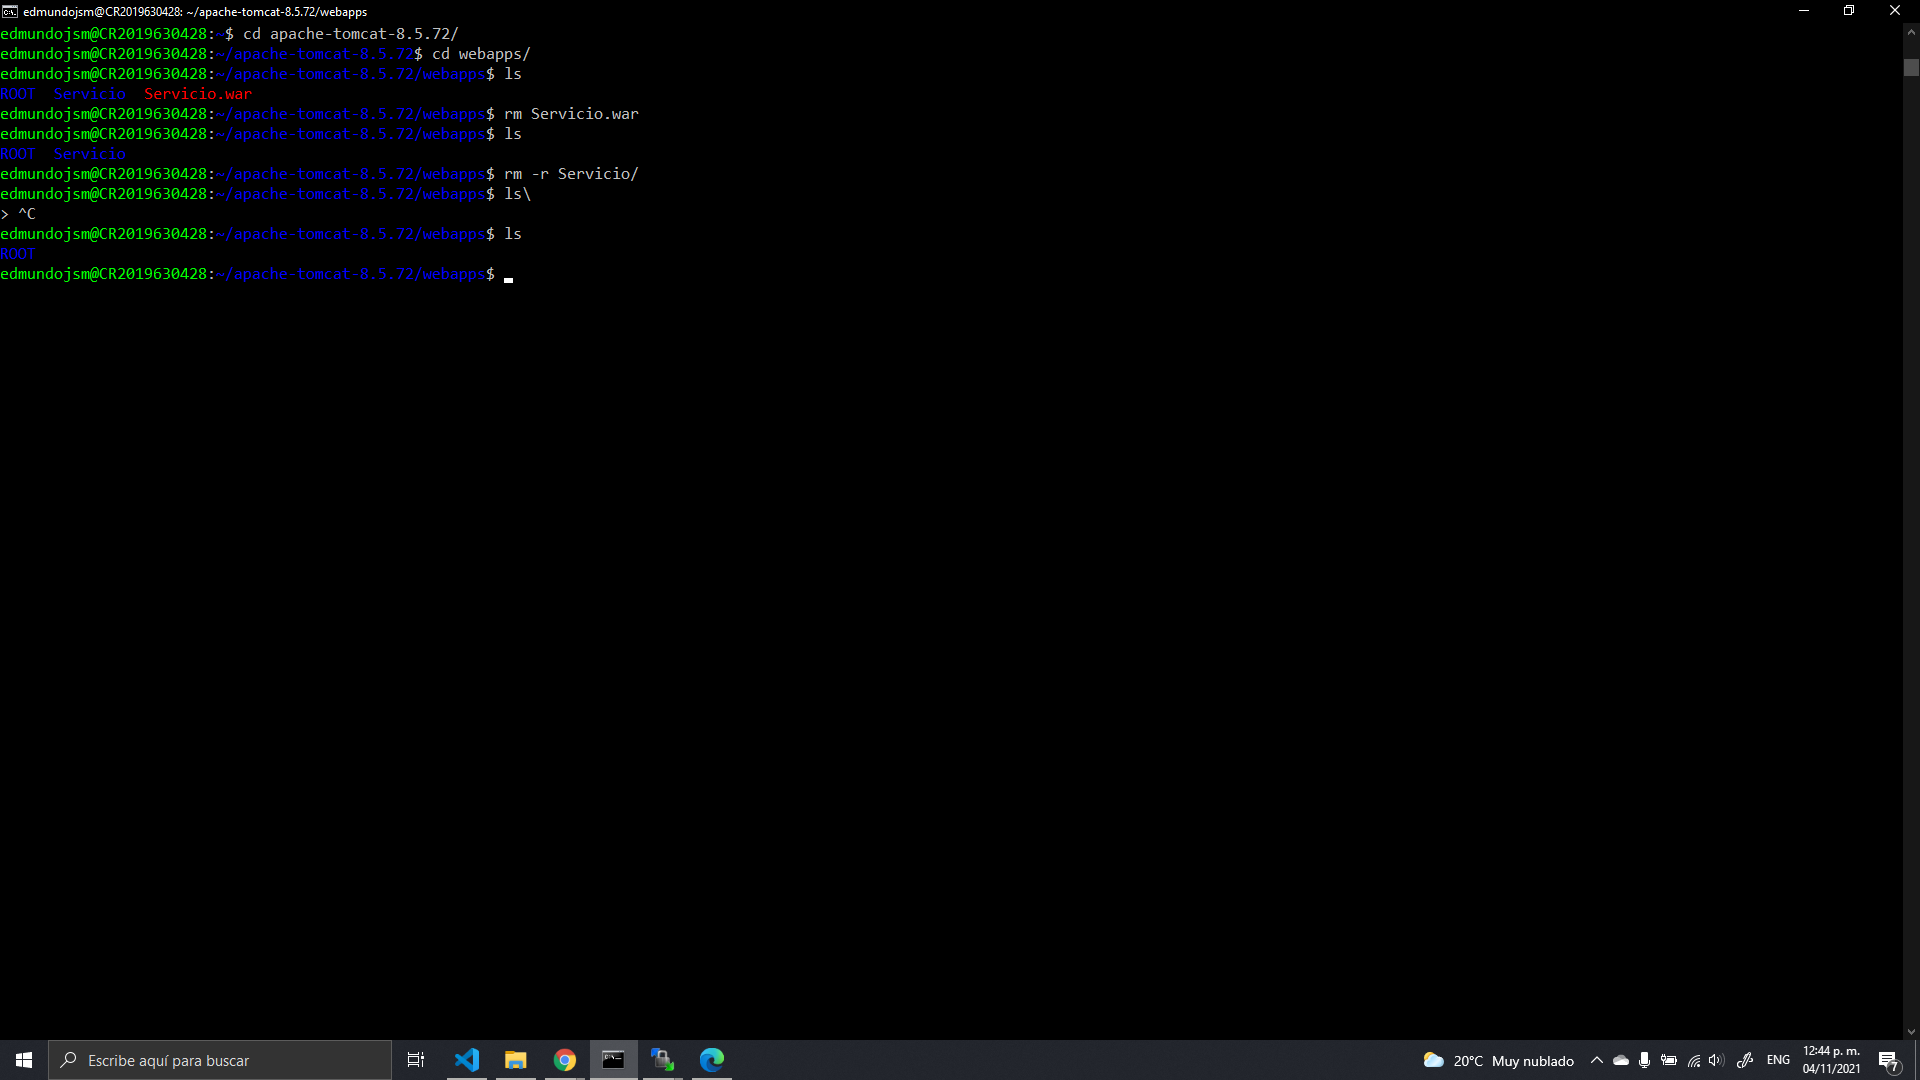
\includegraphics[scale=0.34]{resources/sreviciodelete.png}
			\caption{Carpeta Servicio y Servicio.war eliminado de webapps .}\label{fig:picture}
		\end{figure}
		\begin{figure}[H]
			\centering
			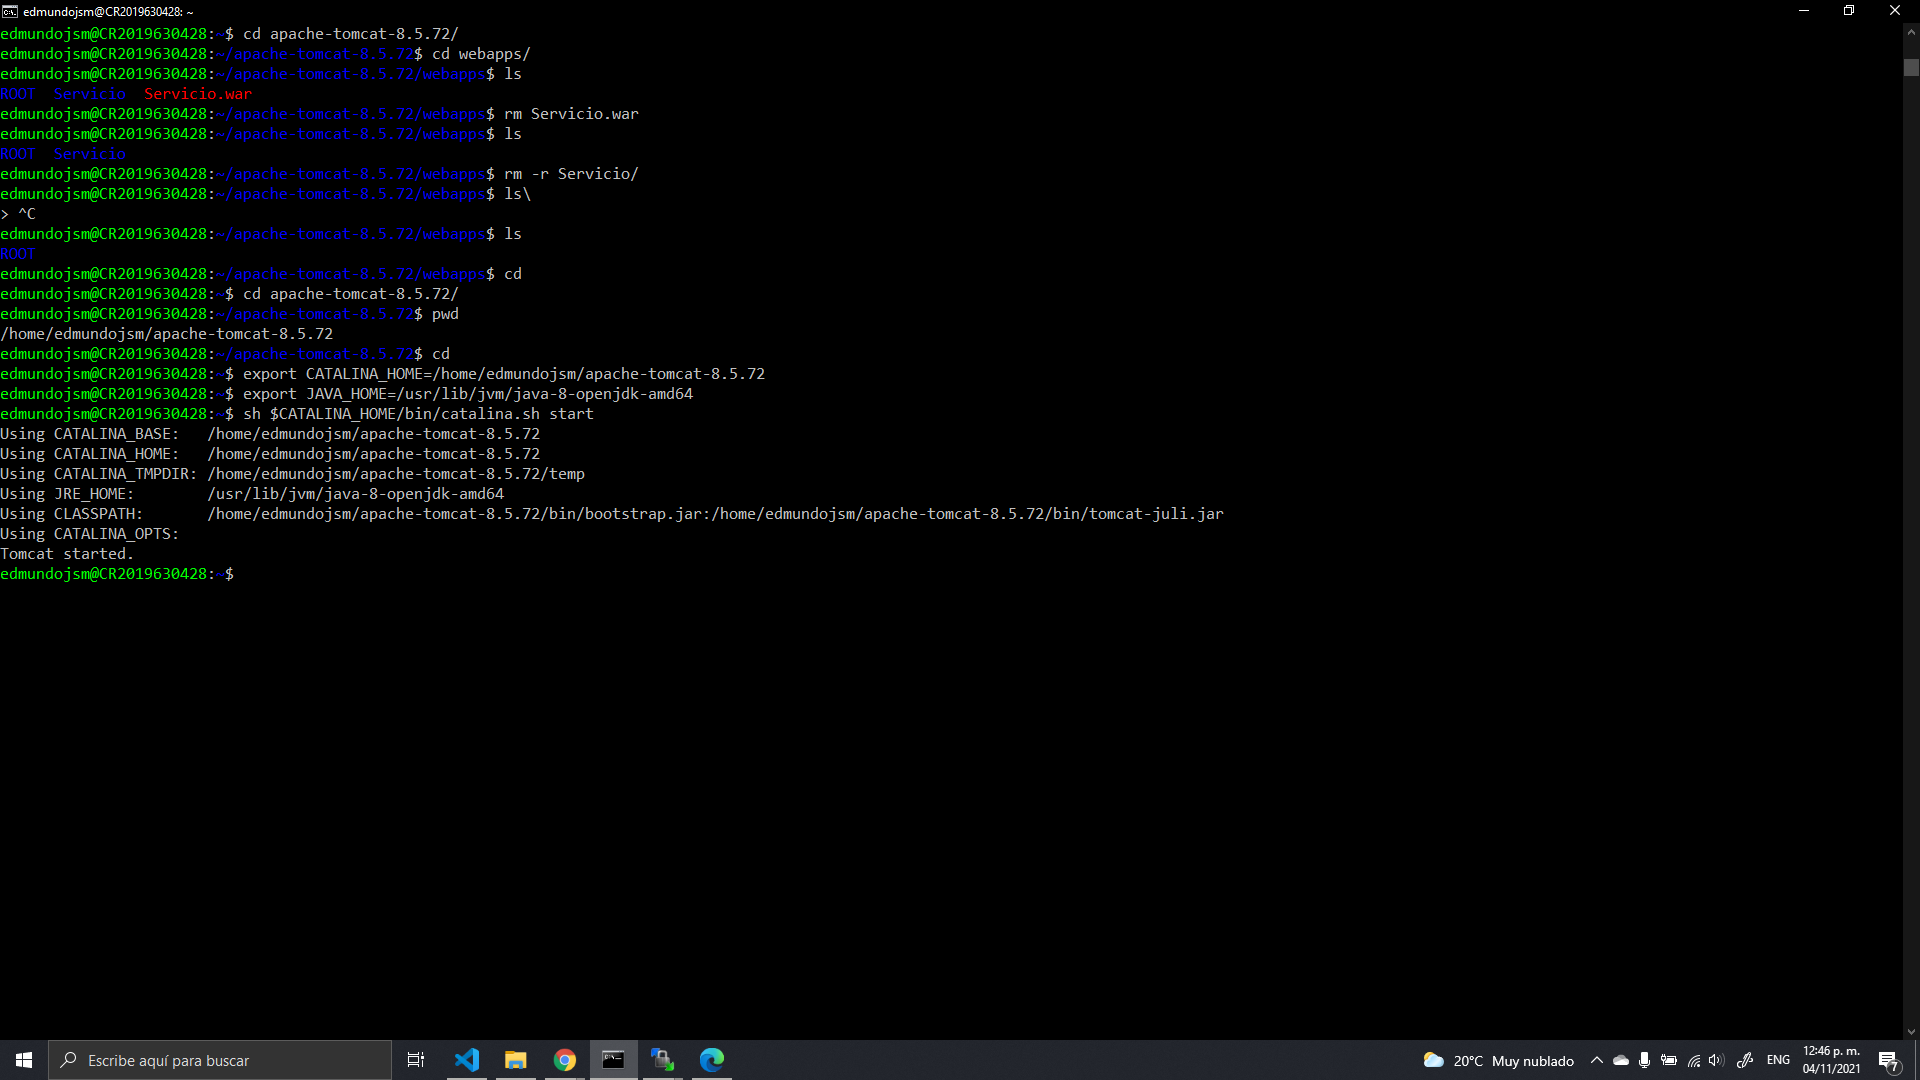
\includegraphics[scale=0.34]{resources/tomcatready.png}
			\caption{Variables de entorno asignadas y Tomcat corriendo.}\label{fig:picture}
		\end{figure}
		Después nos toca compilar el servicio, generar el .war y copiarlo a la carpeta webapps para poder tener el servicio en linea usando Tomcat, todo esto se ve en la figura 19, finalmente abrimos la linea de comando de mysql con el usuario hugo para poder ver la información almacenada en la tabla usuarios y comprobar el correcto funcionamiento de la tarea, esto lo podemos ver en la figura 20.
		\begin{figure}[H]
			\centering
			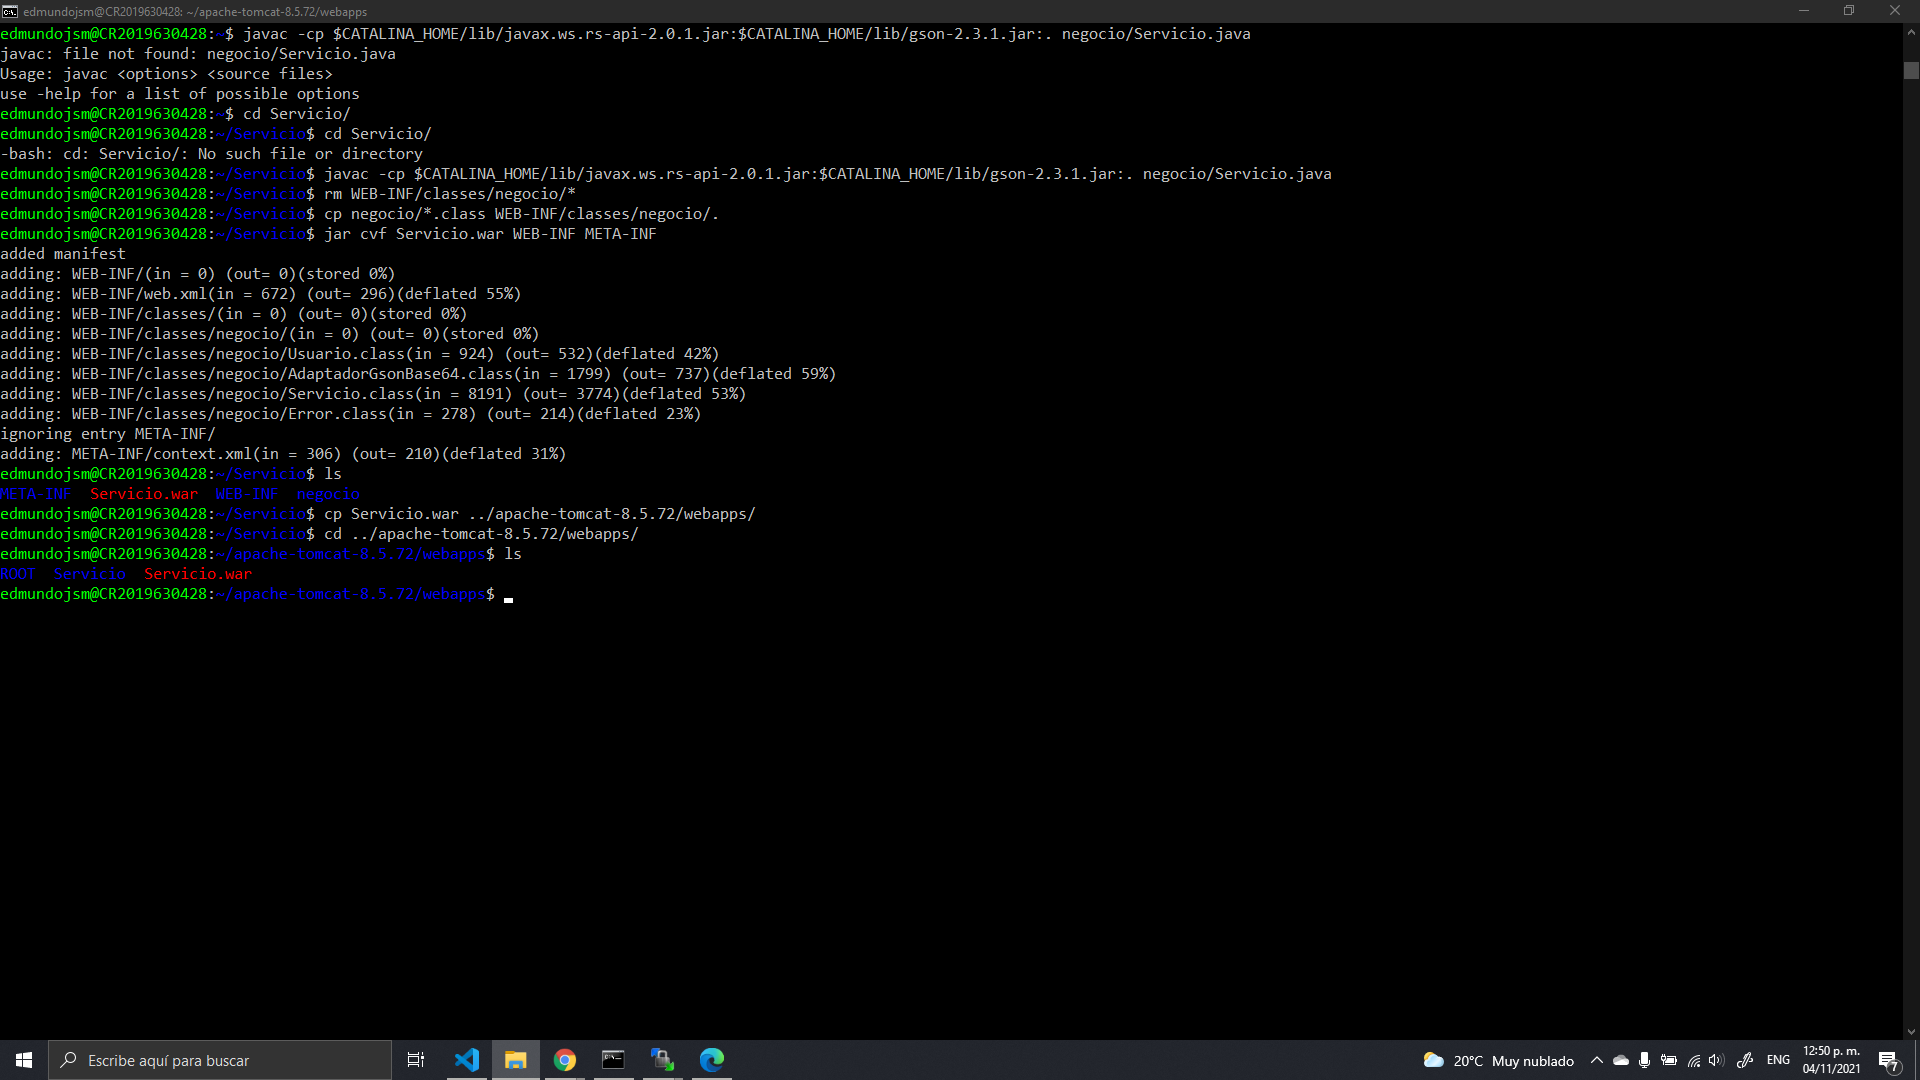
\includegraphics[scale=0.34]{resources/compilacionservicioon.png}
			\caption{Compilación de Servicio y copiado a la carpeta webapps .}\label{fig:picture}
		\end{figure}
		\begin{figure}[H]
			\centering
			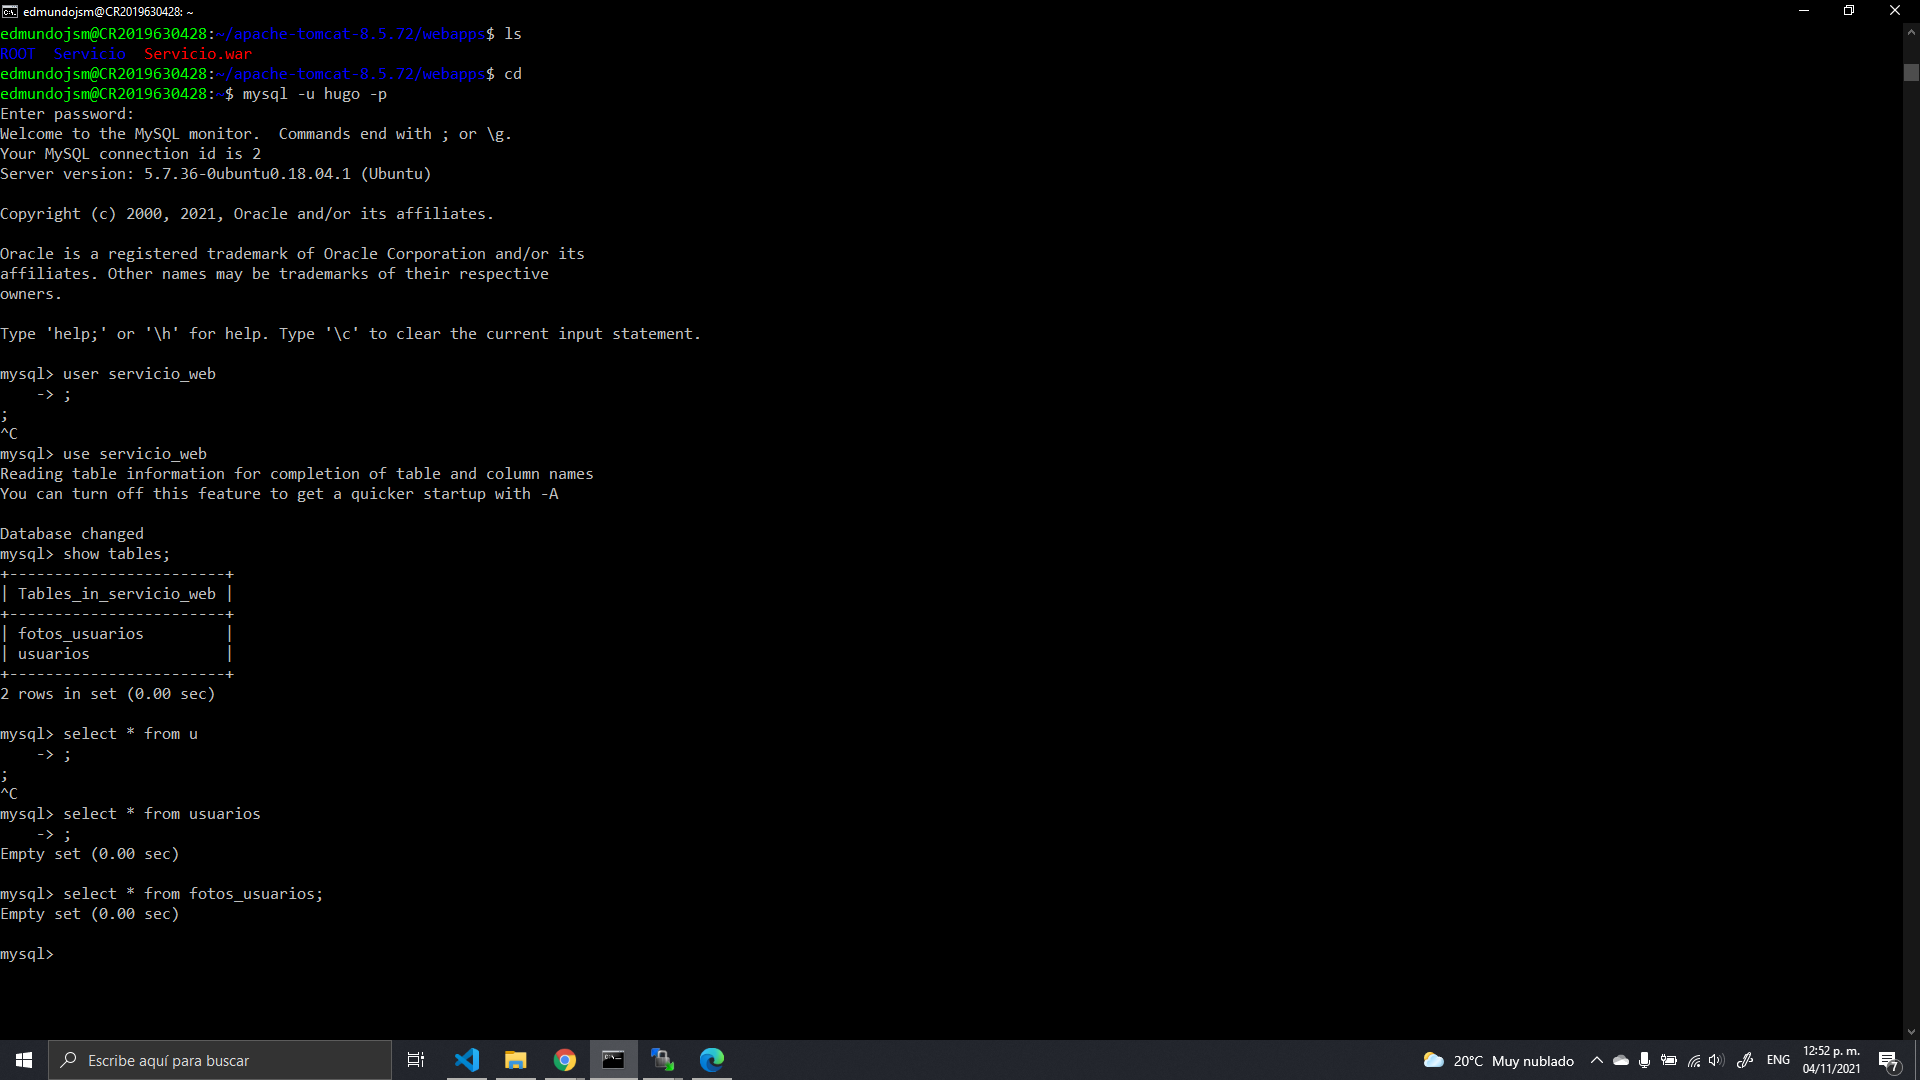
\includegraphics[scale=0.34]{resources/dbempty.png}
			\caption{Estado actual de la base de datos.}\label{fig:picture}
		\end{figure}
		Finalmente la compilación y ejecución del programa Cliente en la computadora local, mencionar que se usa BufferReader en lugar de Scanner ya que este ultimo me arrojaba errores y es que no me dejaba escribir el primer parámetro al momento de querer de dar de alta al usuario, me pasaba inmediatamente al otro campo, también mencionar que es importante compilar pasando el .jar de gson-2.3.1 ya que sin este nos generaría errores y nuestro programa no funcionaria. Todo esto se puede ver en la figura 21.
		\begin{figure}[H]
			\centering
			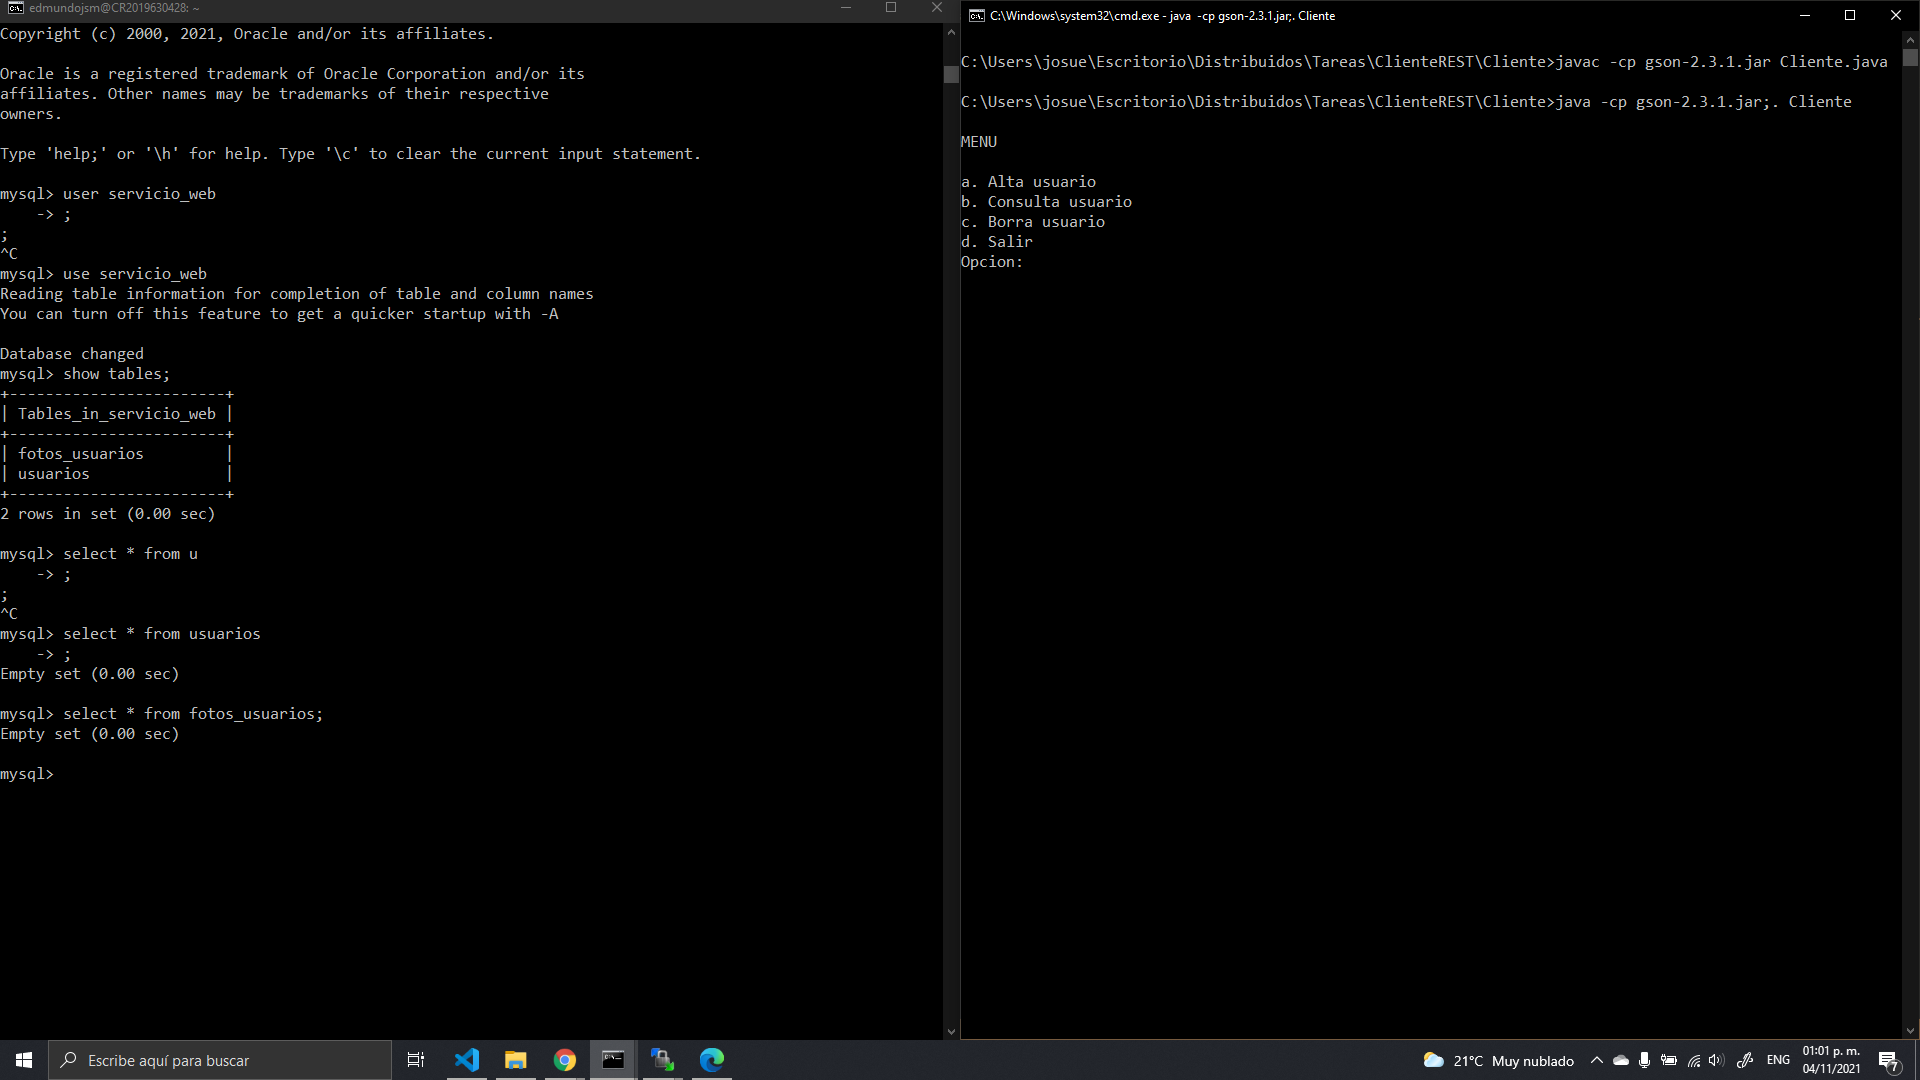
\includegraphics[scale=0.34]{resources/compilacioncliente.png}
			\caption{Estado actual de la base de datos.}\label{fig:picture}
		\end{figure}
		\subsection{Pruebas}
		\subsubsection{Prueba 1}		
 Daremos de alta un nuevo usuario con la información que podemos ver en la figura 22, observar como ahora en la base de datos tenemos un usuario almacenado.
	\begin{figure}[H]
			\centering
			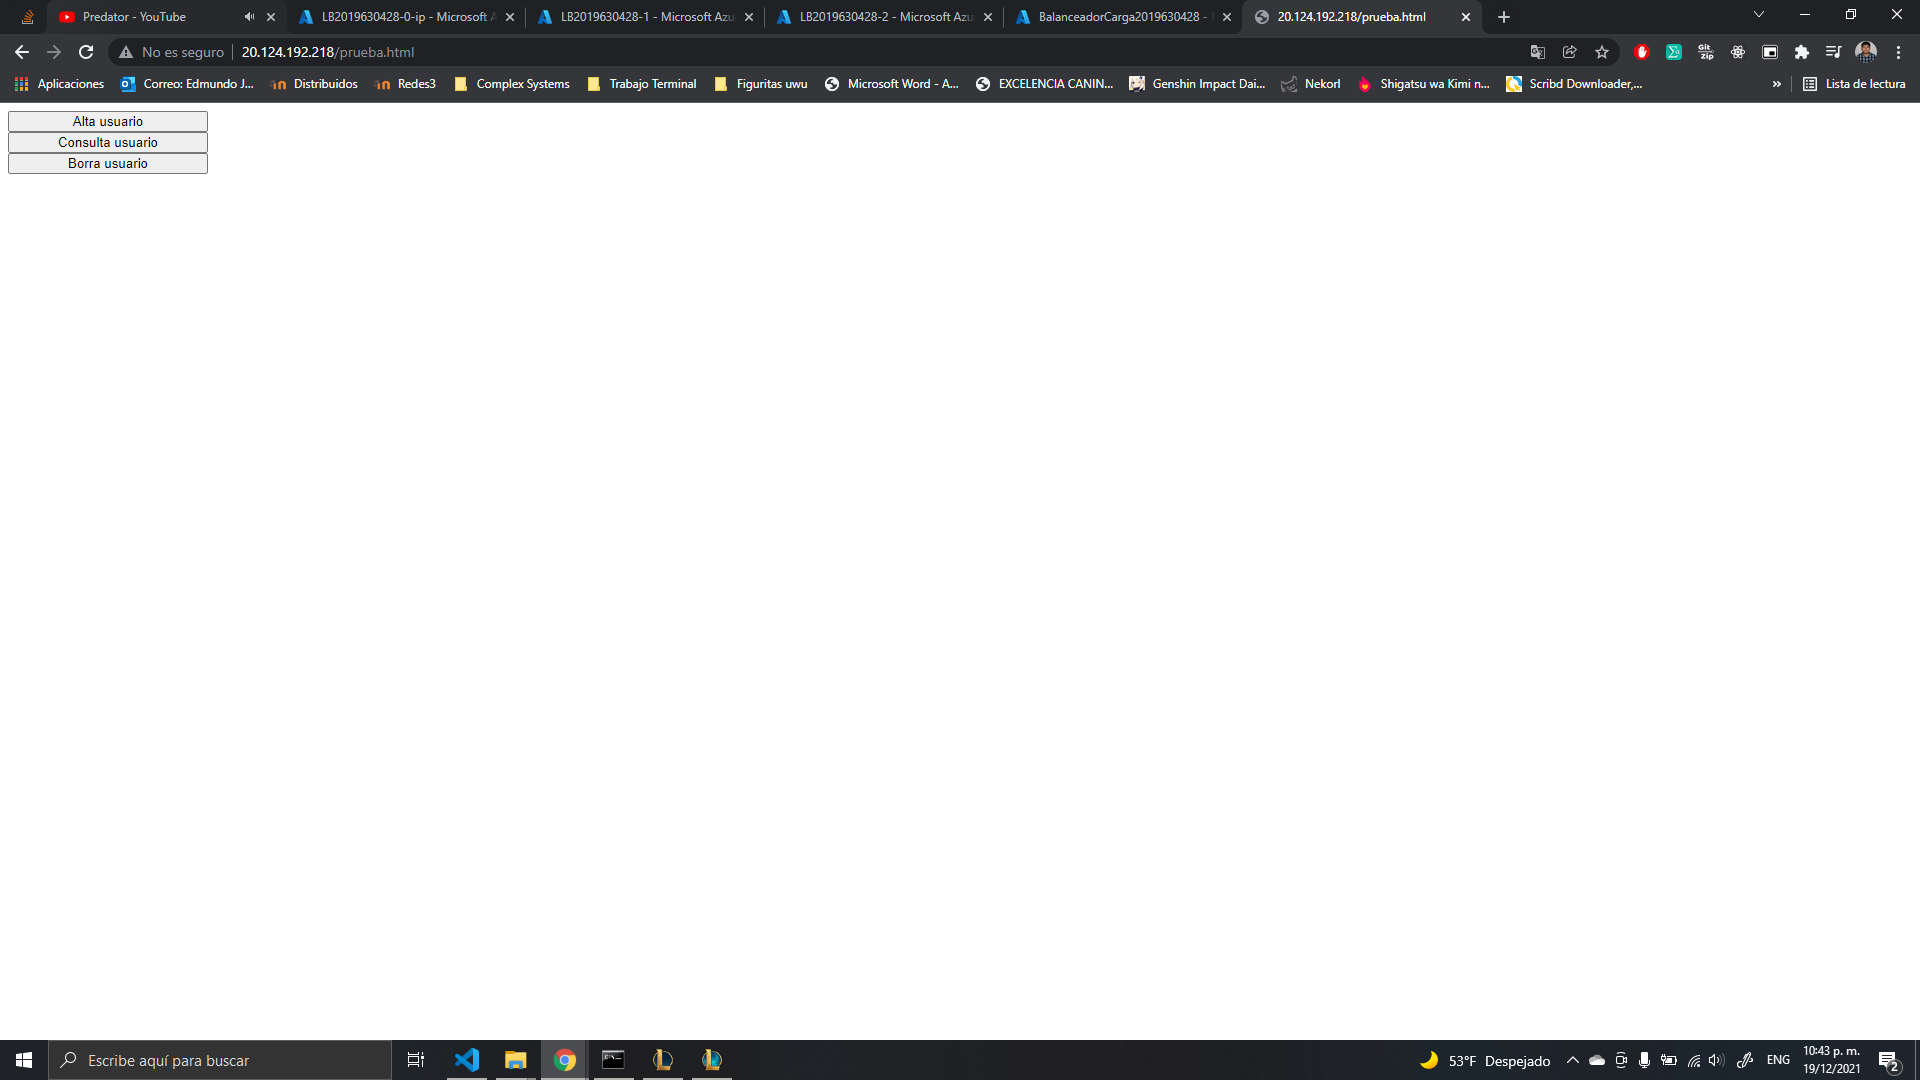
\includegraphics[scale=0.34]{resources/prueba1.png}
			\caption{Prueba 1. Dar de alta a usuario.}\label{fig:picture}
		\end{figure}
		\subsubsection{Prueba 2, 3 y 4}		
Consultaremos al usuario dado de alta en la prueba anterior y cambiaremos algún dato de este, el dato a cambiar sera el teléfono, notar que en la figura 23 vemos con el la base de datos se actualizo el campo, indicando un correcto funcionamiento de la tarea, el la figura 22 vemos los datos que nos regresa el servicio con la modificación del campo teléfono.
		\begin{figure}[H]
			\centering
			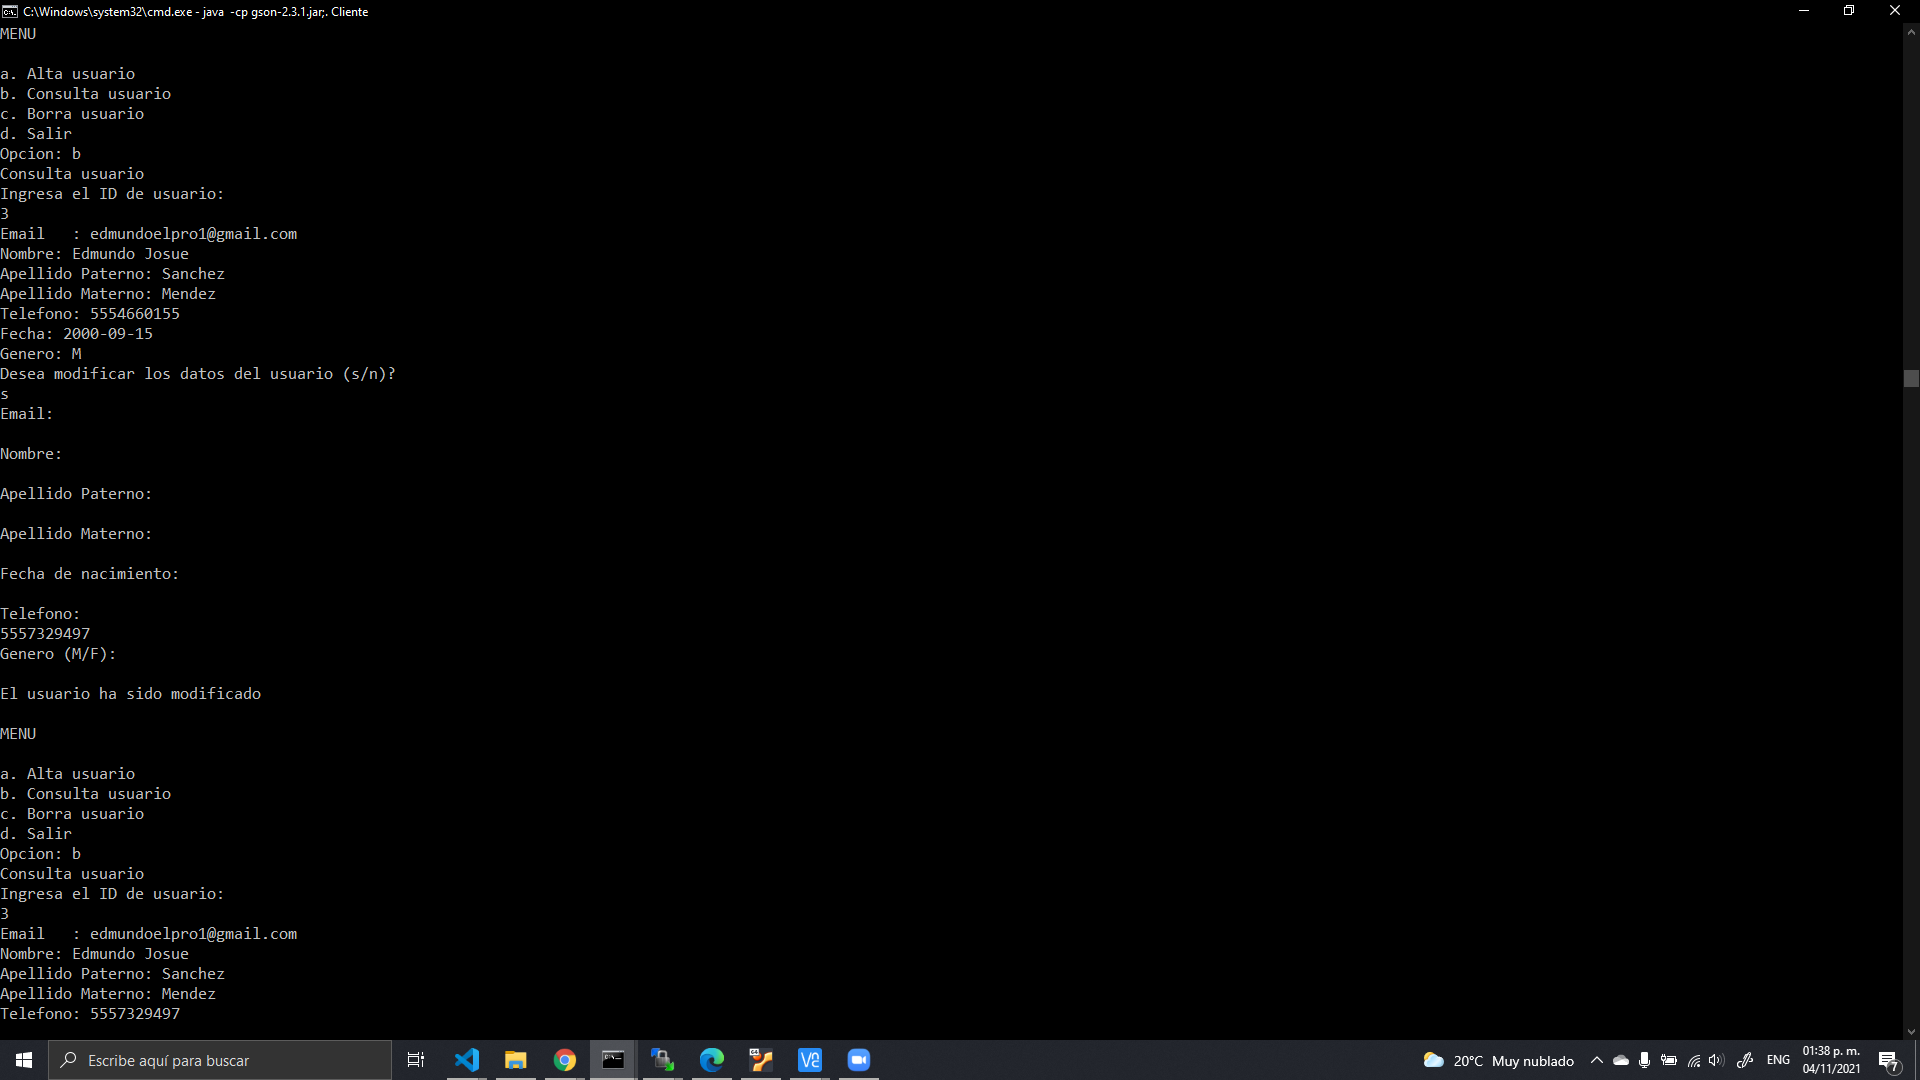
\includegraphics[scale=0.34]{resources/prueba2-3.png}
			\caption{Prueba 2, 3 y 4. Consultar y modificar usuario.}\label{fig:picture}
		\end{figure}
		\begin{figure}[H]
			\centering
			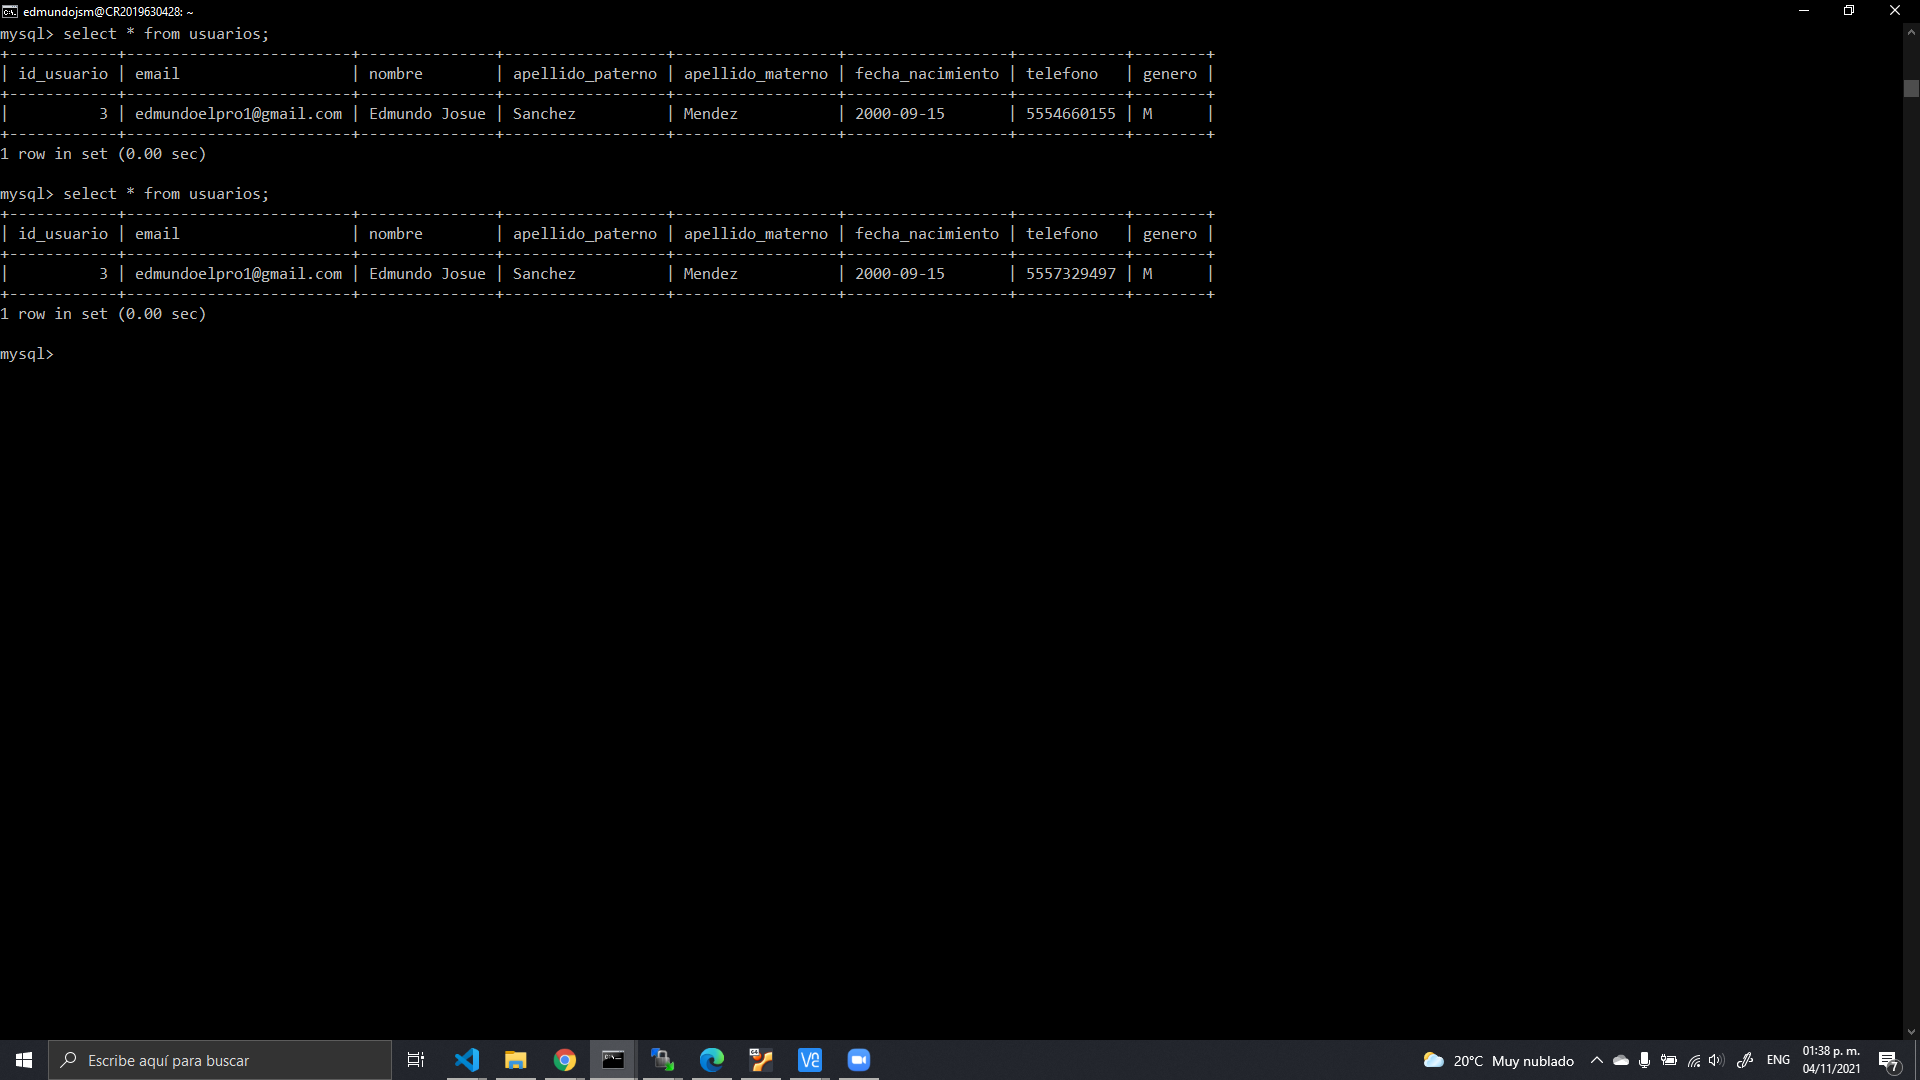
\includegraphics[scale=0.34]{resources/prueba2-3mysql.png}
			\caption{Prueba 2, 3 y 4. Base de datos con los cambios correspondientes.}\label{fig:picture}
		\end{figure}
		\subsubsection{Prueba 5}		
 Intentar borrar un usuario que no exista, como vemos se despliega el mensaje de error indicando que el id no existe.
	\begin{figure}[H]
			\centering
			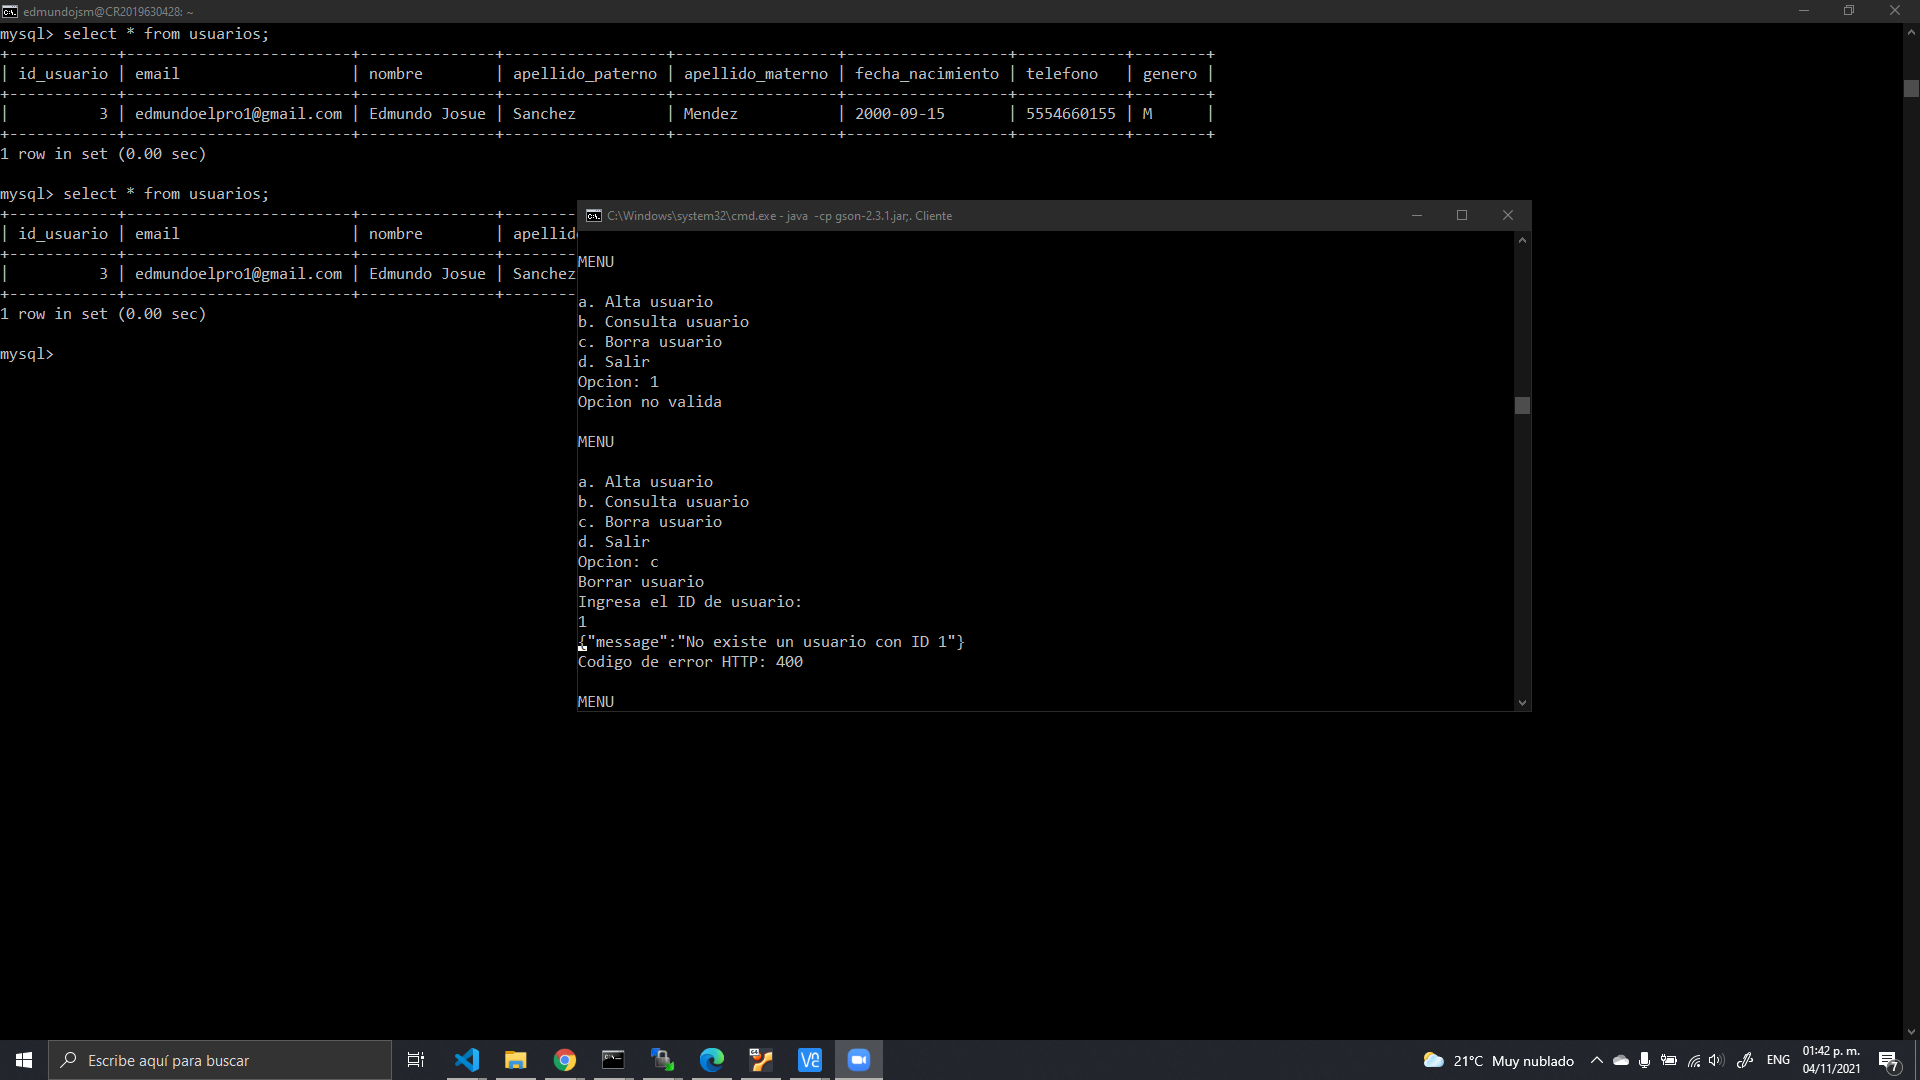
\includegraphics[scale=0.34]{resources/prueba4.png}
			\caption{Prueba 5. Dar de baja a un ID que no existe.}\label{fig:picture}
		\end{figure}		
		\subsubsection{Prueba 6}		
 Borrar el usuario dado de alta en la prueba 1, notar que en la base de datos al momento de seleccionar todos los elementos de la tabla usuario nos arroja que esta esta vacía.
	\begin{figure}[H]
			\centering
			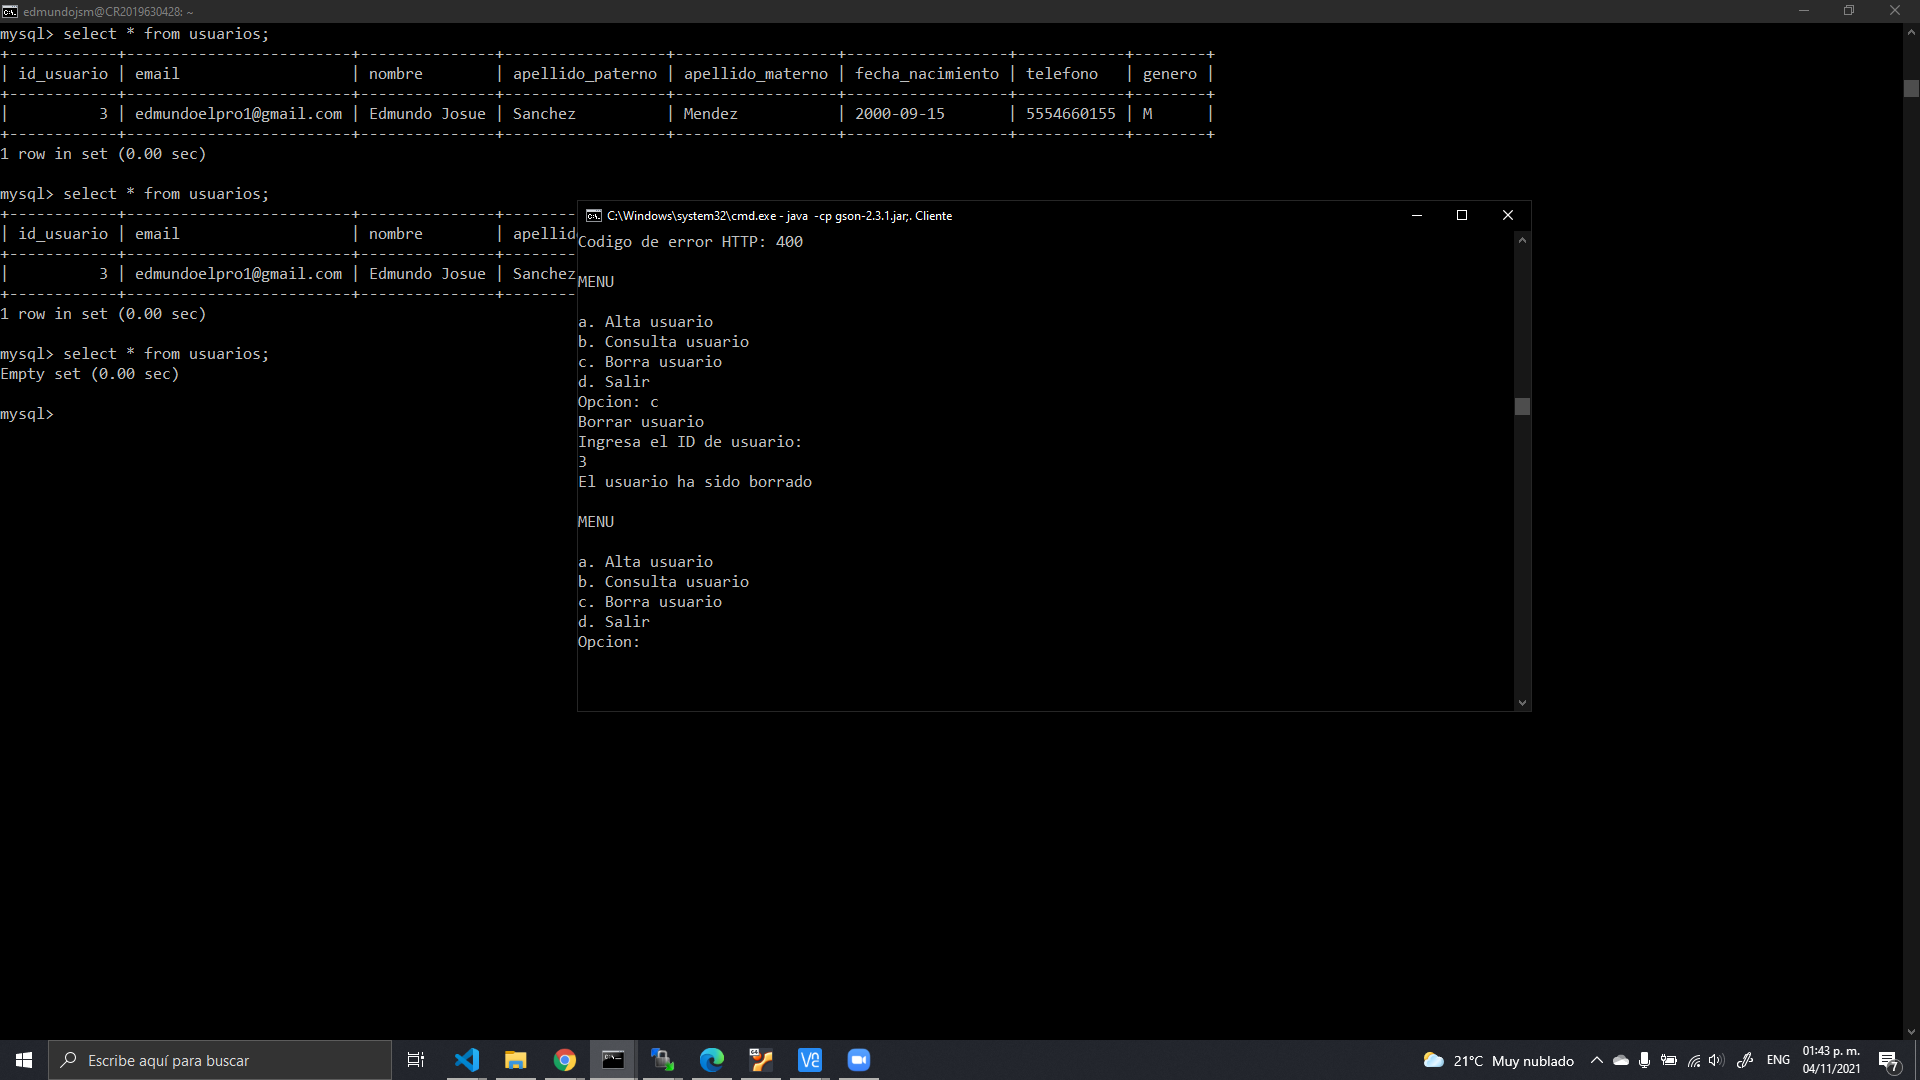
\includegraphics[scale=0.34]{resources/prueba5.png}
			\caption{Prueba 6. Usuario dado de baja.}\label{fig:picture}
		\end{figure}
		\subsubsection{Finalizar programa cliente}		
Se finaliza la ejecución del programa.
	\begin{figure}[H]
			\centering
			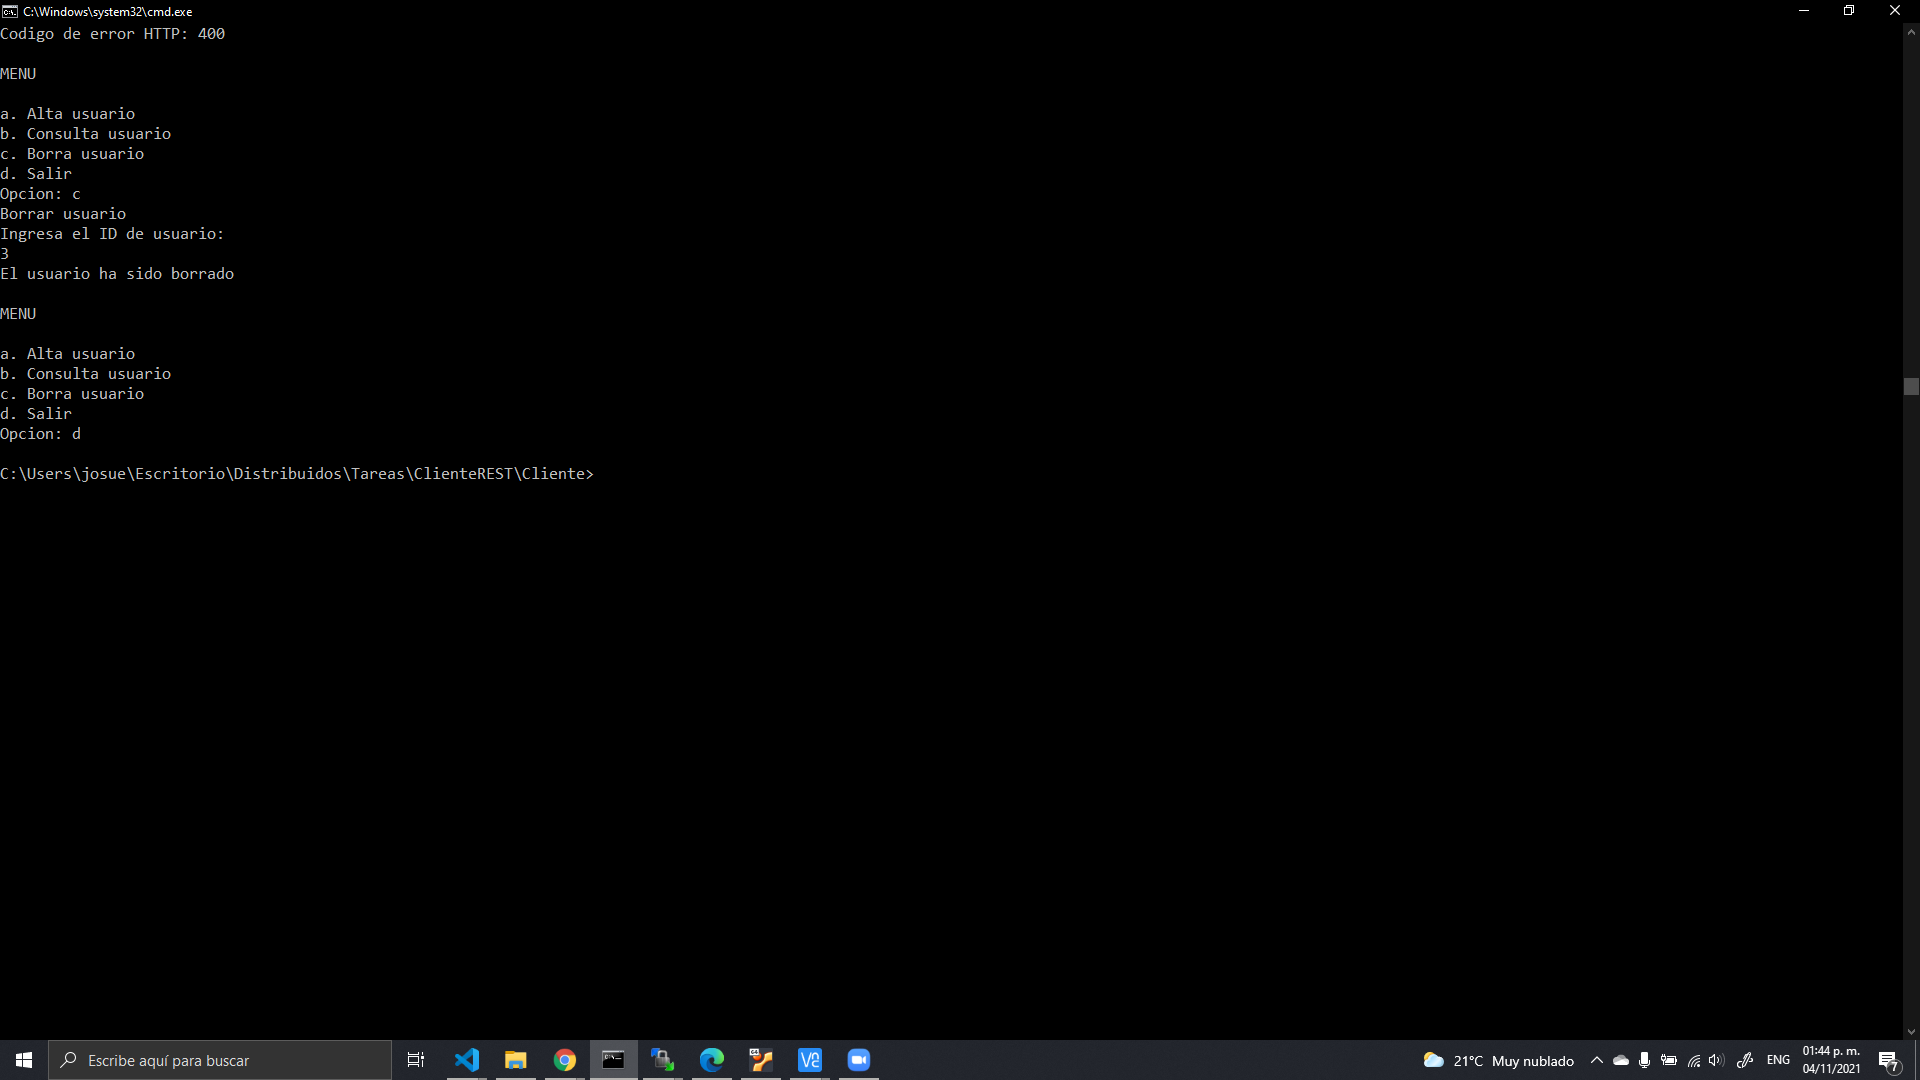
\includegraphics[scale=0.34]{resources/finish.png}
			\caption{Programa finalizado.}\label{fig:picture}
		\end{figure}
		\subsection{Creación de una imagen de la maquina virtual conservando el usuario}
		En este punto tendremos que crear una imagen de la maquina virtual ya que esta tendrá todo lo que instalamos y usamos para esta practica, esto se hace con el fin de usar la imagen para las tareas posteriores, este proceso lo vemos en las figuras 28 a la 31.
		\begin{figure}[H]
			\centering
			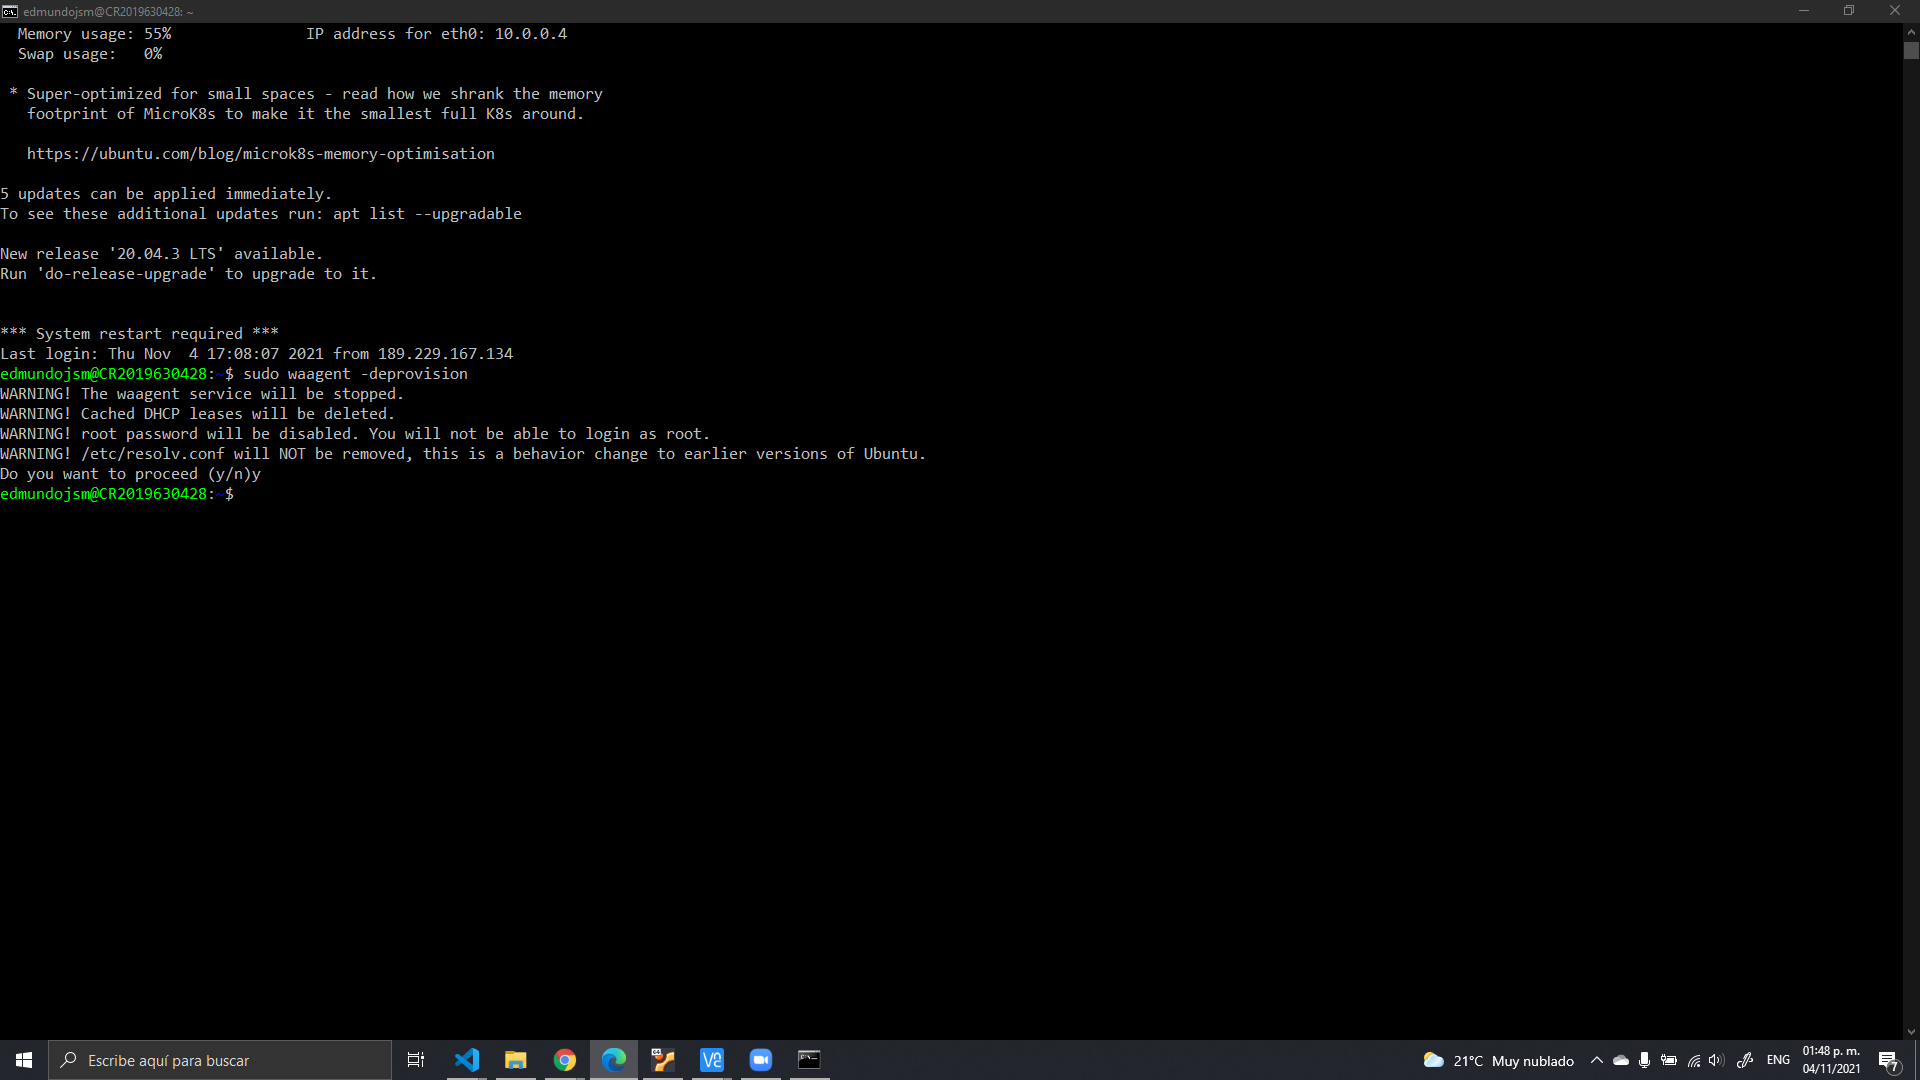
\includegraphics[scale=0.34]{resources/waagent.png}
			\caption{Ejecución del comando sudo waagent -deprovision, esto para crear la imagen con todo y el usuario.}\label{fig:picture}
		\end{figure}
		\begin{figure}[H]
			\centering
			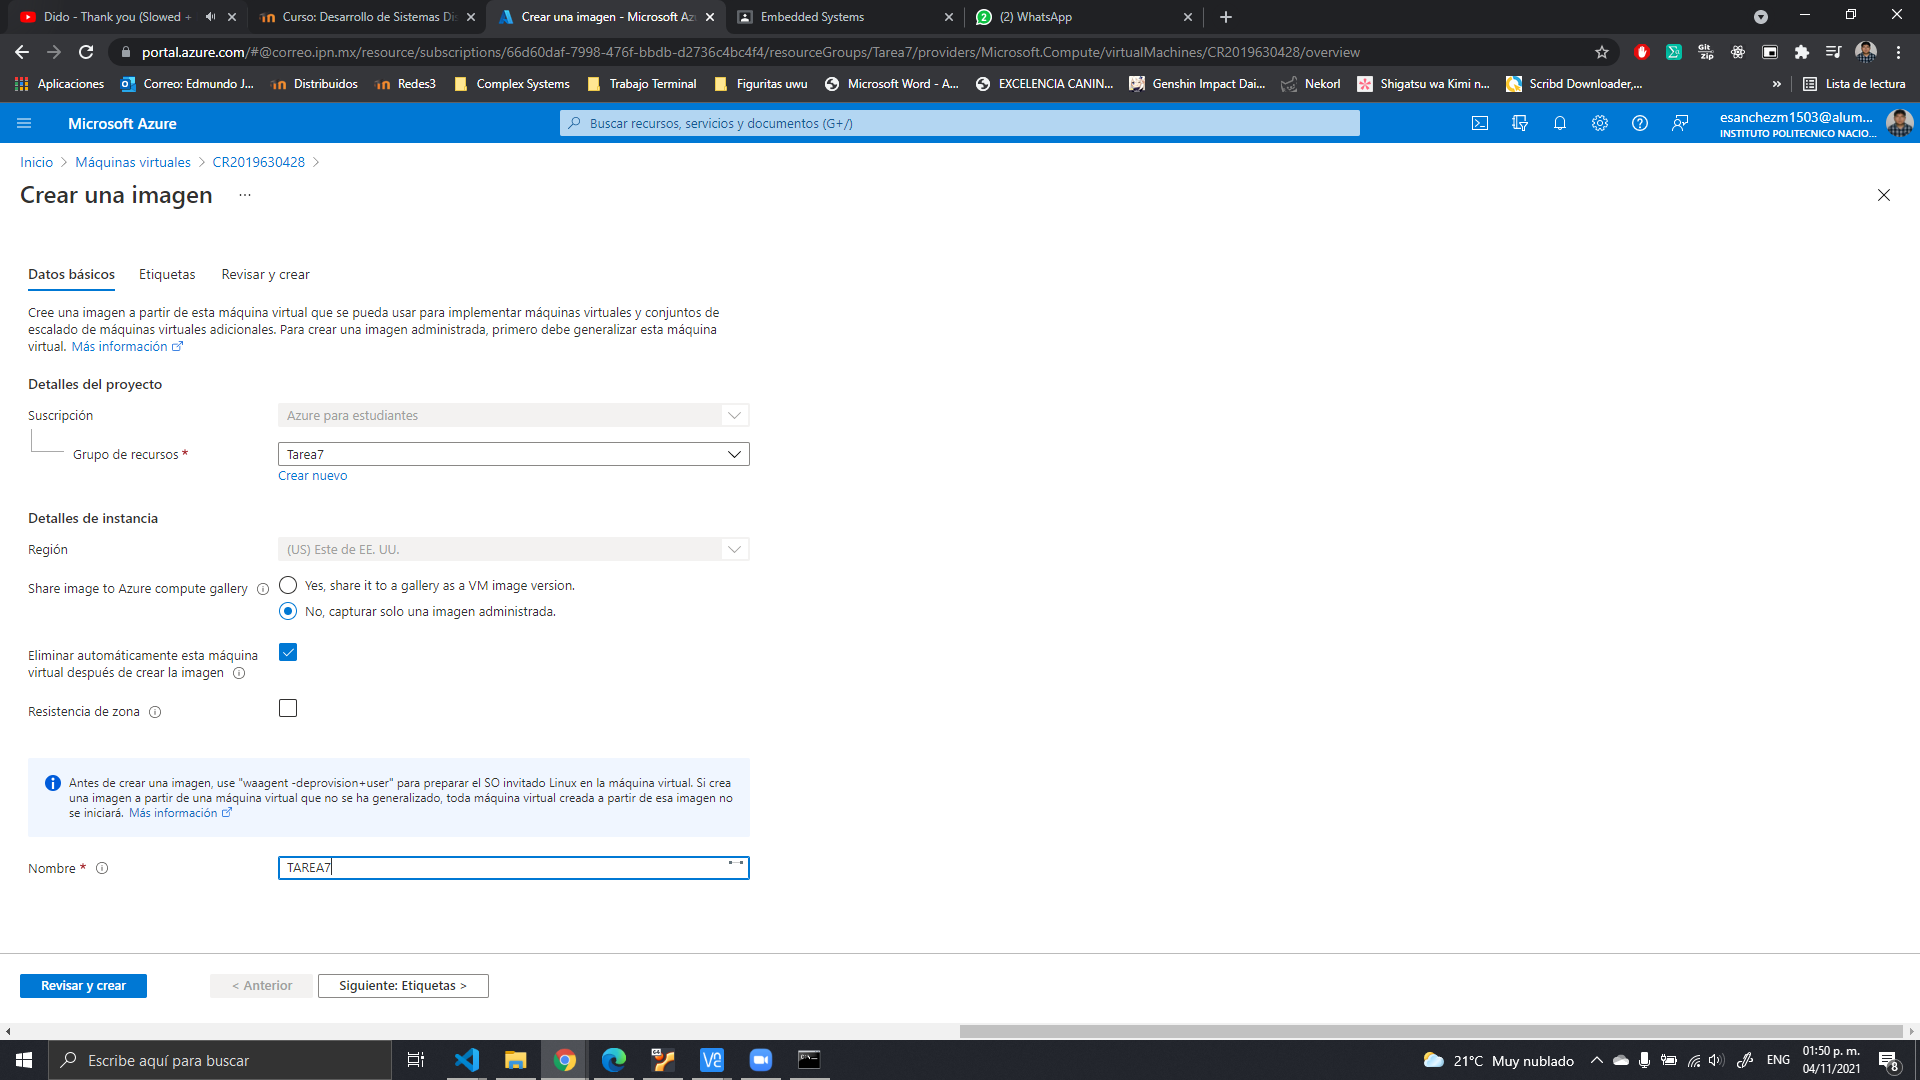
\includegraphics[scale=0.34]{resources/crearimagen.png}
			\caption{Opción seleccionada de eliminar automáticamente esta maquina virtual después de crear la imagen, también elegimos un nombre el cual es TAREA7.}\label{fig:picture}
		\end{figure}
		\begin{figure}[H]
			\centering
			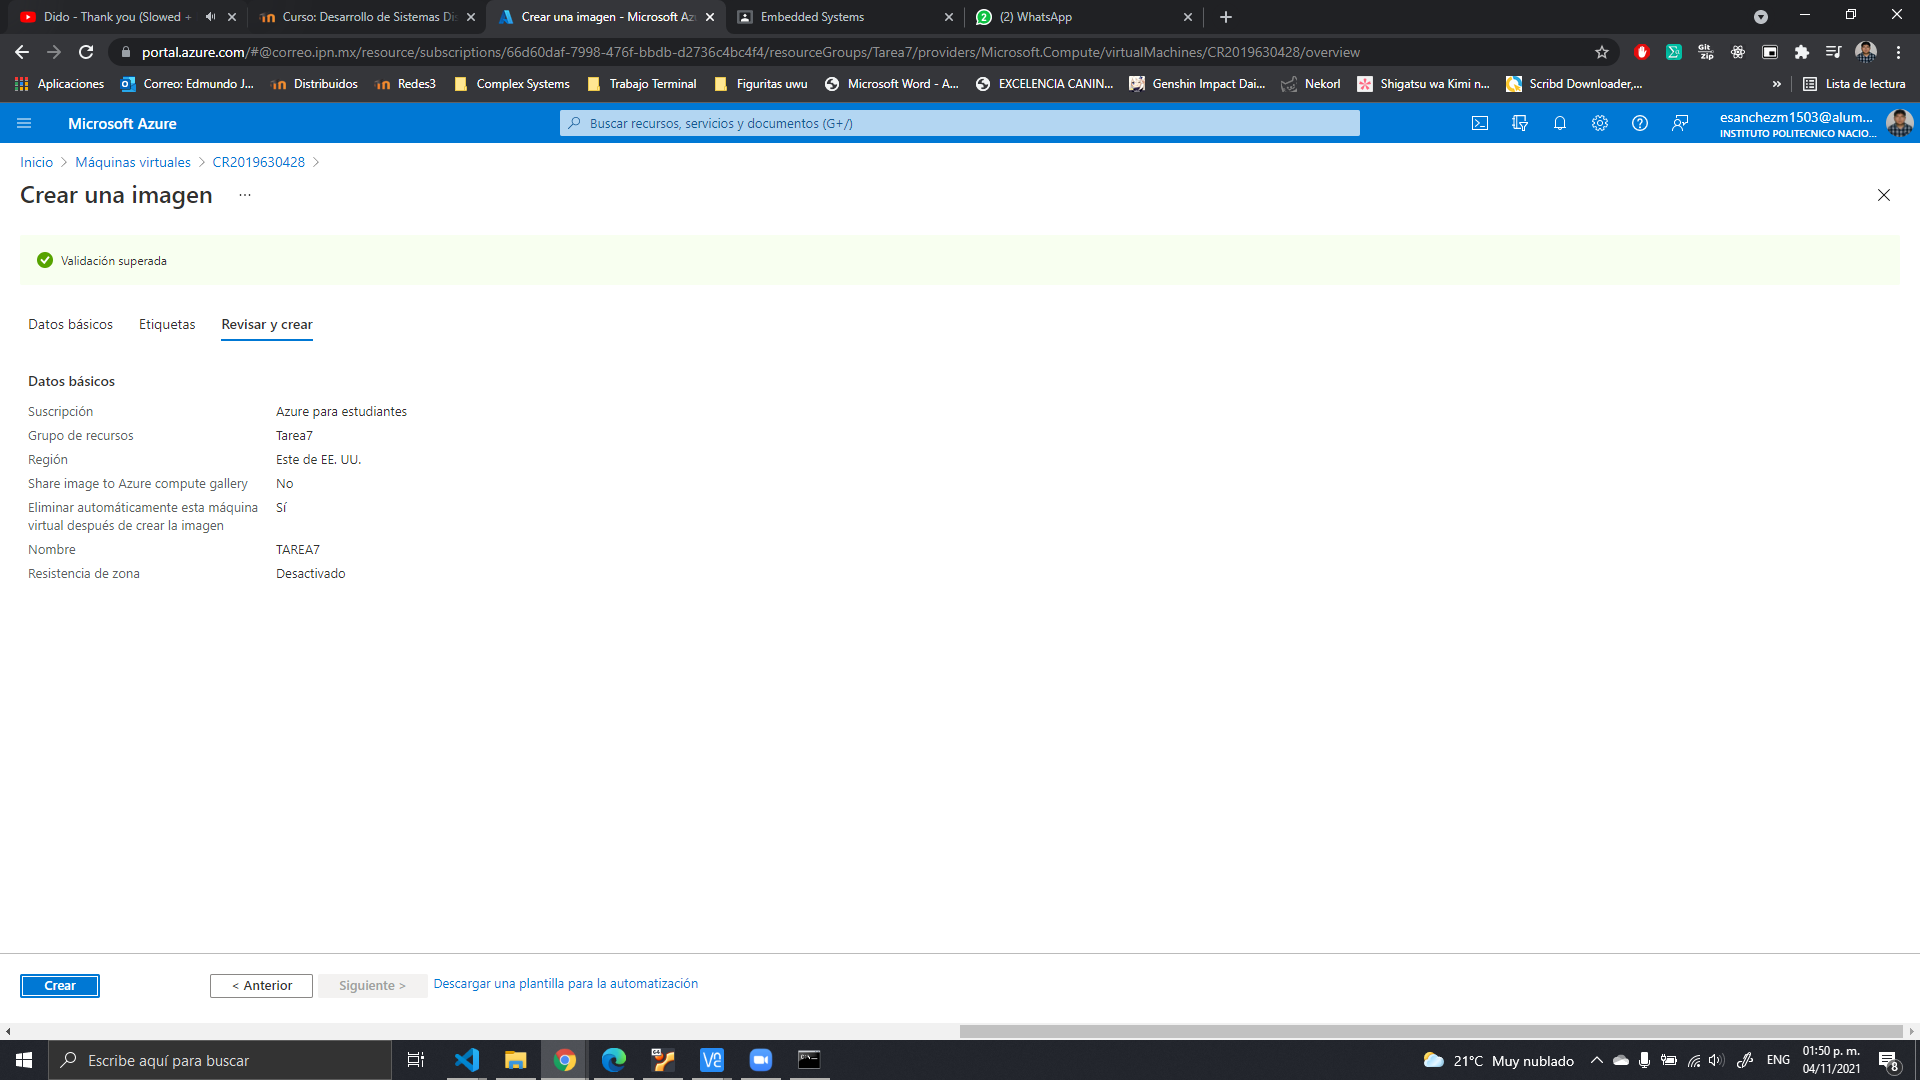
\includegraphics[scale=0.34]{resources/revisarycreaimg.png}
			\caption{Información de la imagen.}\label{fig:picture}
		\end{figure}
		\begin{figure}[H]
			\centering
			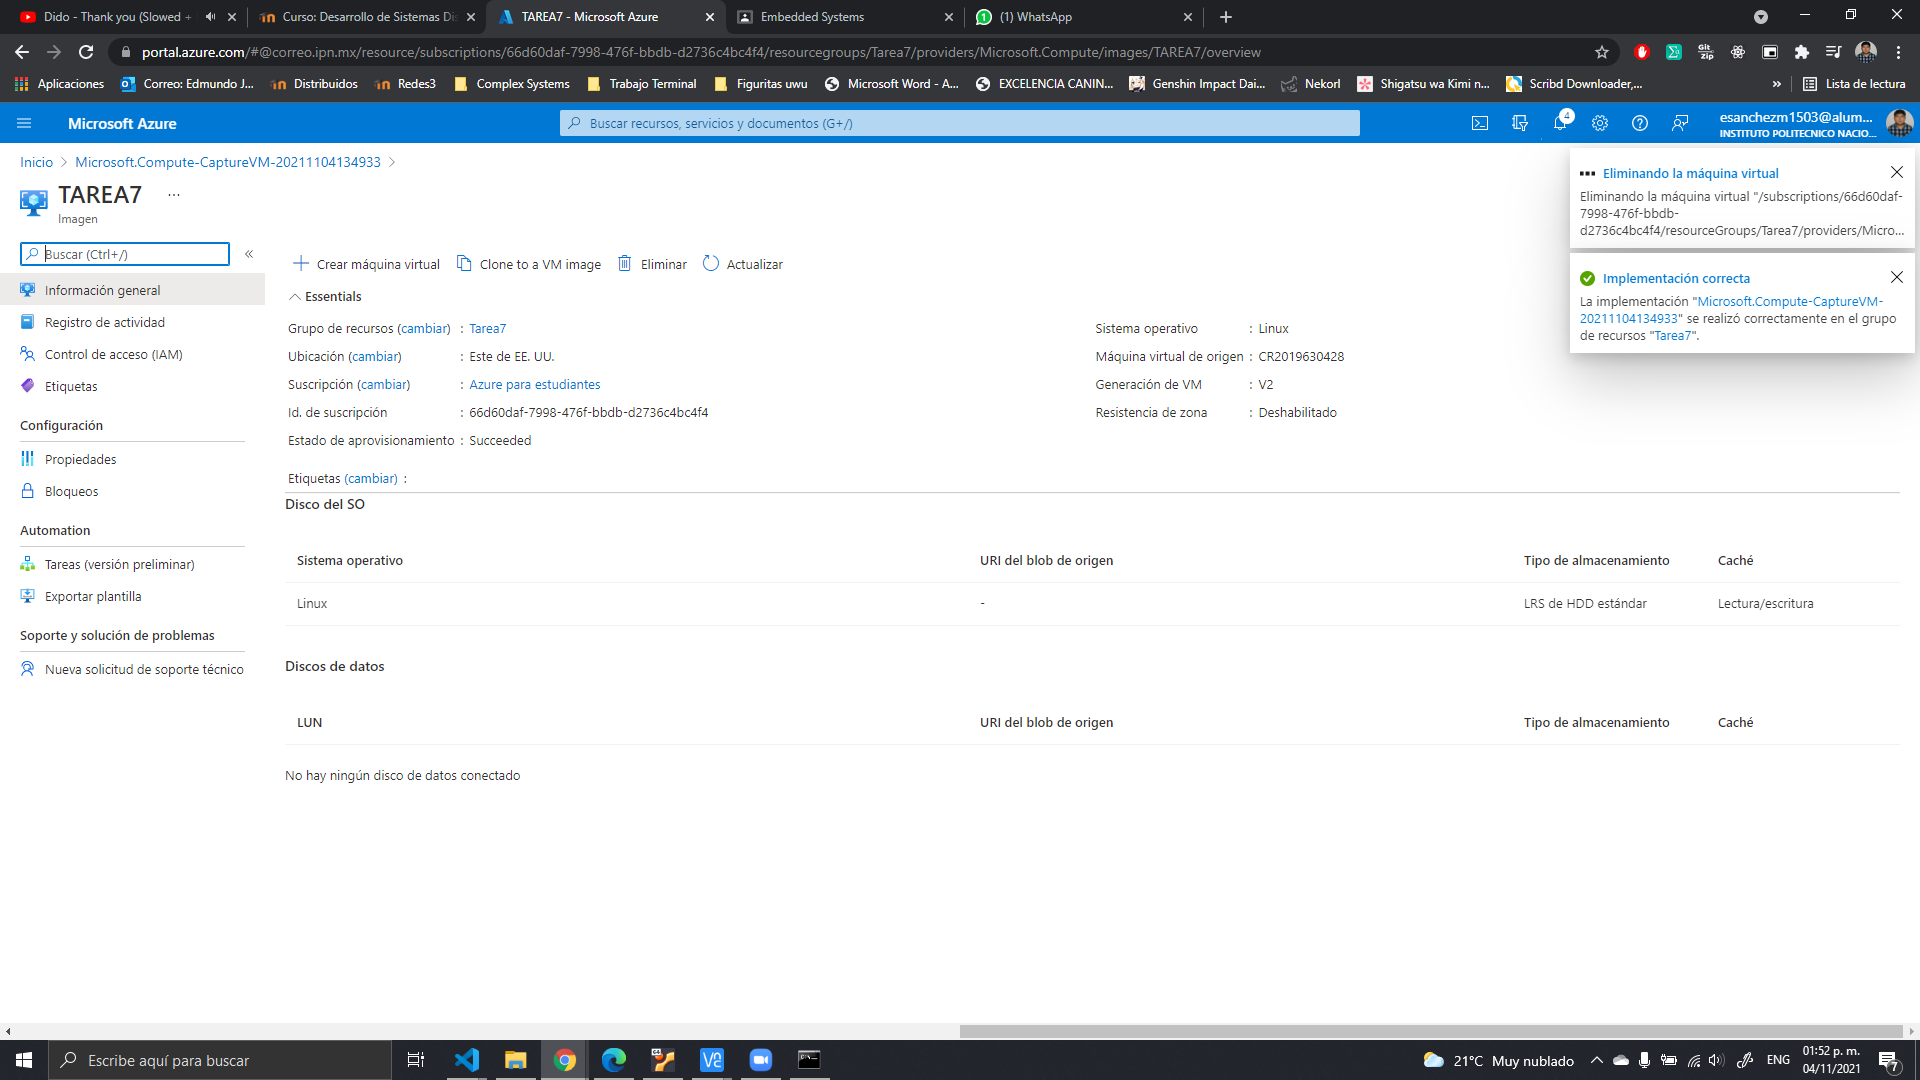
\includegraphics[scale=0.34]{resources/imagenok.png}
			\caption{Imagen creada de manera exitosa.}\label{fig:picture}
		\end{figure}
		
		\section{Conclusiones}
	Al igual que en la tarea anterior observamos el funcionamiento de una aplicación REST, y su comportamiento básico. Solo que en esta ocasión la aplicación que consume REST es una aplicación desarrollada en Java y no es una aplicación WEB, esto nos permite ver la versatilidad de las aplicaciones REST ya que funciona tanto para aplicaciones de escritorio como para aplicaciones en l;a WEB, esto trae como consecuencia el uso muy sencillo y rápido de crear diferentes aplicaciones para que pueden consumir la aplicación REST. En lo que respecta al desarrollo del código para al cliente fue muy sencillo ya que durante la ESCOM se hacen programas de manera local con la misma lógica, así que solo fue traer los conocimientos ya obtenidos y vaciarlos en la tarea, evidentemente apegandonos a lo solicitado para la entrega de esta. 
\end{document}
